\documentclass[a4paper, 12pt]{article}

\usepackage[english, russian]{babel}
\usepackage[T1, T2A]{fontenc}
\usepackage[utf8]{inputenc}
\usepackage{graphicx}
\usepackage{import}
\usepackage{subcaption}
\usepackage{float}
\usepackage{geometry}
\usepackage{amsmath}
\usepackage{amsfonts}
\usepackage{tabu}
\usepackage{booktabs}
\usepackage[dvipsnames]{xcolor}
\usepackage[colorlinks]{hyperref}
\usepackage{indentfirst}
\usepackage{listings}
\usepackage{src/title}

\geometry{left=2cm, right=2cm, bottom=2cm, top=2cm}

\hypersetup{
linkcolor=blue,
filecolor=magenta,
urlcolor=cyan
}

\definecolor{codegreen}{rgb}{0,0.6,0}
\definecolor{codegray}{rgb}{0.5,0.5,0.5}
\definecolor{codepurple}{rgb}{0.58,0,0.82}
\definecolor{backcolour}{rgb}{0.95,0.95,0.92}

\lstdefinestyle{codestyle}{
backgroundcolor=\color{backcolour},
commentstyle=\color{codegreen},
keywordstyle=\color{magenta},
numberstyle=\tiny\color{codegray},
stringstyle=\color{codepurple},
basicstyle=\ttfamily\footnotesize,
breakatwhitespace=false,
breaklines=true,
captionpos=b,
keepspaces=true,
numbers=left,
numbersep=5pt,
showspaces=false,
showstringspaces=false,
showtabs=false,
tabsize=2
}

\lstset{style=codestyle}
\lstset{extendedchars=\true}

%%%%%%%%%%%%%%%%%%%%%%%%%%%%%%%%%%%%%%%%%%%%%%%%
%% Титульный лист
%%%%%%%%%%%%%%%%%%%%%%%%%%%%%%%%%%%%%%%%%%%%%%%%
\title{
Робот с дифференциальным приводом
}

\author{Мостафа Эхаб Ахмед Абделвахаб Мохамед}
\affil{503341}

\author{Ануфриев Андрей Сергеевич}
\affil{465029}

\supervisor{Овчаров Алексей Олегович}

\abstract{
В работе исследовано движение робота с дифференциальным приводом при использовании двух способов управления: P-регулятора и тангенциального регулятора. Для обоих законов управления построены модели в Simulink, проведены эксперименты на реальном роботе EV3 и выполнено сравнение экспериментальных и модельных траекторий. Отдельно рассмотрены одиночные переходы в заданные точки и последовательное движение по квадратной траектории.
}

\keywords{
дифференциальный привод; одометрия; P-регулятор; тангенциальный регулятор; Simulink; EV3
}

\date{12.05.2026}

%%%%%%%%%%%%%%%%%%%%%%%%%%%%%%%%%%%%%%%%%%%%%%%%
% Начало документа
%%%%%%%%%%%%%%%%%%%%%%%%%%%%%%%%%%%%%%%%%%%%%%%%
\begin{document}
\maketitle

\section{Постановка задачи}

Цель работы --- построить математическую модель робота с дифференциальным приводом, реализовать два закона управления движением к цели, сравнить экспериментальные данные с моделированием в Simulink и оценить, насколько хорошо модель описывает поведение реального робота.

Для достижения цели в работе были поставлены следующие задачи:
\begin{enumerate}
\item изучить кинематическую модель робота с дифференциальным приводом;
\item реализовать одометрию для вычисления координат робота по данным энкодеров;
\item реализовать P-регулятор и тангенциальный регулятор для движения к целевой точке;
\item построить обе схемы управления в Simulink;
\item провести эксперименты при движении из точки $(0,0)$ в точки $(1,0)$, $(0,1)$, $(-1,0)$ и $(0,-1)$;
\item провести эксперимент с движением по квадратной траектории;
\item обработать данные и построить графики для каждого регулятора отдельно и для их общего сравнения;
\item проанализировать расхождения между моделью и экспериментом и сделать выводы.
\end{enumerate}

\section{Теоретическая часть}

\subsection{Математическая модель робота}

Положение робота на плоскости задаётся координатами $x$, $y$ и углом ориентации $\theta$. Кинематическая модель робота с дифференциальным приводом имеет вид
\begin{equation}
\dot{x} = v\cos\theta,
\end{equation}
\begin{equation}
\dot{y} = v\sin\theta,
\end{equation}
\begin{equation}
\dot{\theta} = \omega,
\end{equation}
где $v$ --- линейная скорость центра робота, а $\omega$ --- угловая скорость.

Если за малый промежуток времени левое и правое колёса повернулись на углы $\Delta\psi_l$ и $\Delta\psi_r$, то путь центра робота и изменение угла можно вычислить по формулам
\begin{equation}
\Delta L = \frac{(\Delta\psi_l + \Delta\psi_r)r}{2},
\end{equation}
\begin{equation}
\Delta\theta = \frac{(\Delta\psi_r - \Delta\psi_l)r}{B},
\end{equation}
где $r$ --- радиус колеса, $B$ --- база робота.

В работе использовались параметры робота EV3: $r = 29$ мм и $B = 120$ мм. Эти же значения применялись в программе и в модели Simulink.

\subsection{Одометрия}

Одометрия позволяет оценивать текущее положение робота по приращениям углов колёс. На каждом шаге вычисляются приращения координат
\begin{equation}
\Delta x = \Delta L \cos\theta,
\end{equation}
\begin{equation}
\Delta y = \Delta L \sin\theta,
\end{equation}
\begin{equation}
\Delta\theta = \frac{(\Delta\psi_r - \Delta\psi_l)r}{B},
\end{equation}
после чего координаты обновляются:
\begin{equation}
x_i = x_{i-1} + \Delta x,
\end{equation}
\begin{equation}
y_i = y_{i-1} + \Delta y,
\end{equation}
\begin{equation}
\theta_i = \theta_{i-1} + \Delta\theta.
\end{equation}

В модели такой подход работает хорошо, но в реальном эксперименте ошибка постепенно накапливается. Причина не только в проскальзывании, но и в неидеальности моторов, дискретности энкодеров, несимметрии колёс и в том, что сама модель является упрощённой.

\subsection{P-регулятор}

Для движения в точку $(x_g, y_g)$ вводятся расстояние до цели
\begin{equation}
\rho = \sqrt{(x_g - x)^2 + (y_g - y)^2},
\end{equation}
азимут на цель
\begin{equation}
\psi = \mathrm{atan2}(y_g - y, x_g - x),
\end{equation}
и курсовая ошибка
\begin{equation}
\alpha = \psi - \theta.
\end{equation}

В P-регуляторе используются выражения
\begin{equation}
U_s = K_s\rho,
\end{equation}
\begin{equation}
U_r = K_r\alpha,
\end{equation}
а сигналы на моторы задаются как
\begin{equation}
U_{left} = U_s - U_r,
\end{equation}
\begin{equation}
U_{right} = U_s + U_r.
\end{equation}

Такой регулятор прост по структуре, но форма траектории зависит от соотношения двух управляющих частей: поступательной $U_s = K_s \rho$ и поворотной $U_r = K_r \alpha$. Если в начале движения угол ошибки $\alpha$ велик, то робот одновременно получает команду и на движение вперёд, и на поворот. Из-за этого он не доворачивается на месте, а начинает идти по дуге. Чем больше отношение $K_s \rho / K_r \alpha$ в начальный момент, тем сильнее робот уходит вперёд до полного доворота, и тем шире получается траектория.

\begin{figure}[H]
    \centering
    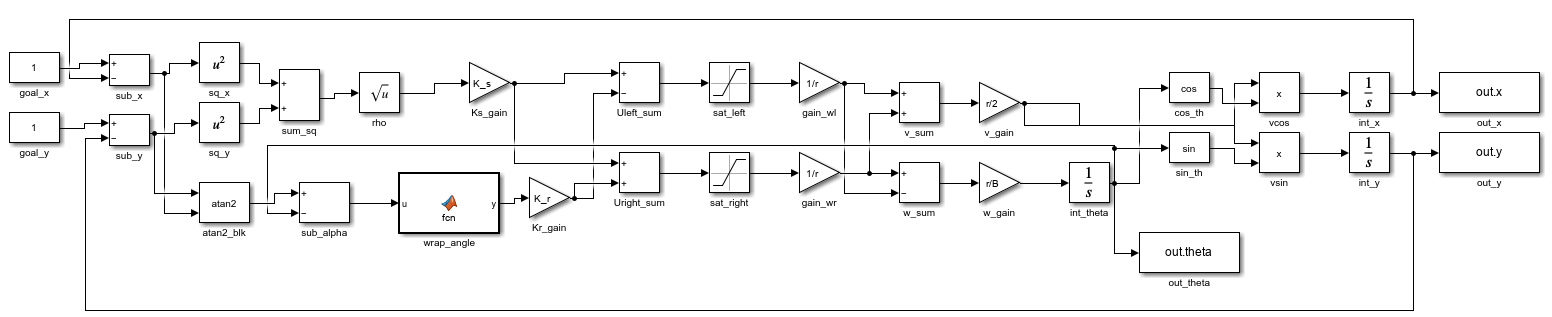
\includegraphics[width=0.9\textwidth]{images/p_shema}
    \caption{Схема P-регулятора в Simulink}
    \label{fig:p_shema}
\end{figure}

\subsection{Тангенциальный регулятор}

В тангенциальном регуляторе линейная и угловая составляющие задаются формулами
\begin{equation}
v_{goal} = K_1\rho\cos(\alpha),
\end{equation}
\begin{equation}
\omega_{goal} = K_1\cos(\alpha)\sin(\alpha) + K_2\alpha.
\end{equation}

Сигналы на моторы задаются как
\begin{equation}
U_{left} = v_{goal} - \omega_{goal},
\end{equation}
\begin{equation}
U_{right} = v_{goal} + \omega_{goal}.
\end{equation}

У тангенциального регулятора форма траектории определяется иначе. Линейная скорость содержит множитель $\cos(\alpha)$, то есть при большой ошибке по углу движение вперёд автоматически уменьшается. Если $\alpha \approx \pm \frac{\pi}{2}$, то $\cos(\alpha)$ близок к нулю, и робот почти не едет вперёд, а в основном доворачивается. Поэтому траектория получается более компактной, а боковой уход в начале движения меньше, чем у P-регулятора.

\begin{figure}[H]
    \centering
    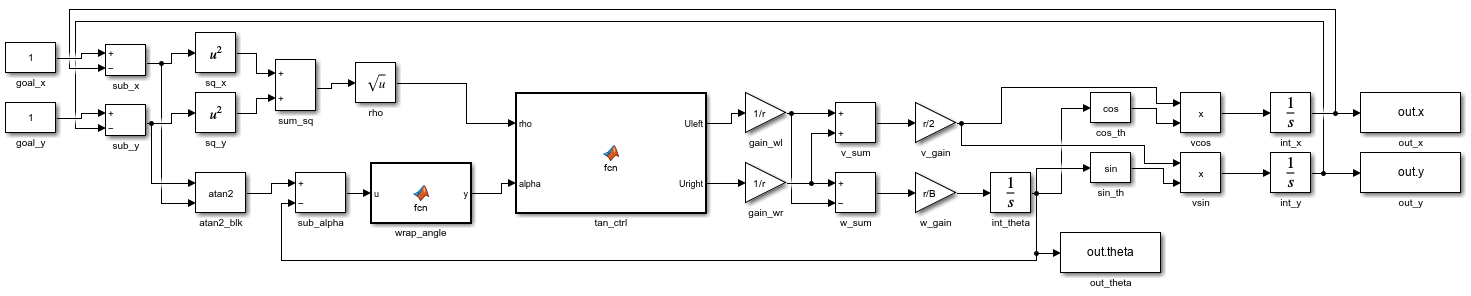
\includegraphics[width=0.9\textwidth]{images/t_shema}
    \caption{Схема тангенциального регулятора в Simulink}
    \label{fig:t_shema}
\end{figure}

\section{Результаты экспериментов}

В этой части сначала отдельно рассматриваются результаты для P-регулятора, затем для тангенциального регулятора, а после этого приводится их общее сравнение. Такой порядок позволяет сначала оценить поведение каждого регулятора самого по себе, а потом сравнить их между собой.

\subsection{P-регулятор}

\subsubsection*{Одиночные переходы}

\begin{figure}[H]
    \centering
    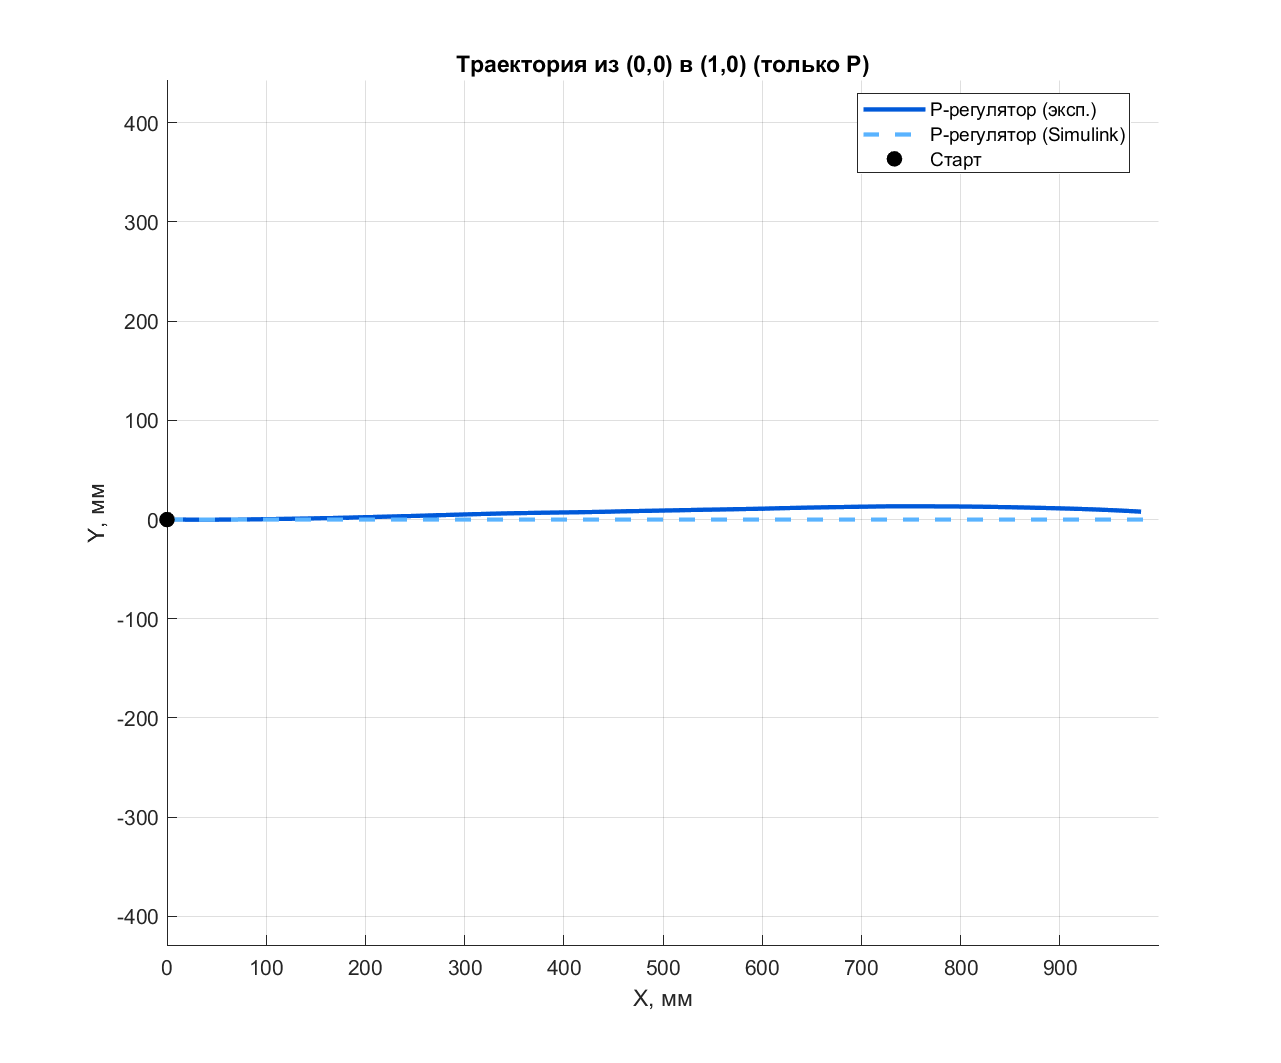
\includegraphics[width=0.82\textwidth]{../graphics/point_P_1.png}
    \caption{P-регулятор: движение из $(0,0)$ в $(1,0)$}
    \label{fig:p_only_1}
\end{figure}

При движении в точку $(1,0)$ траектория близка к прямой, так как начальная ошибка по углу мала. В этом случае сигнал $U_r$ невелик, и робот в основном движется вперёд. Поэтому эксперимент и модель совпадают здесь лучше всего.

\begin{figure}[H]
    \centering
    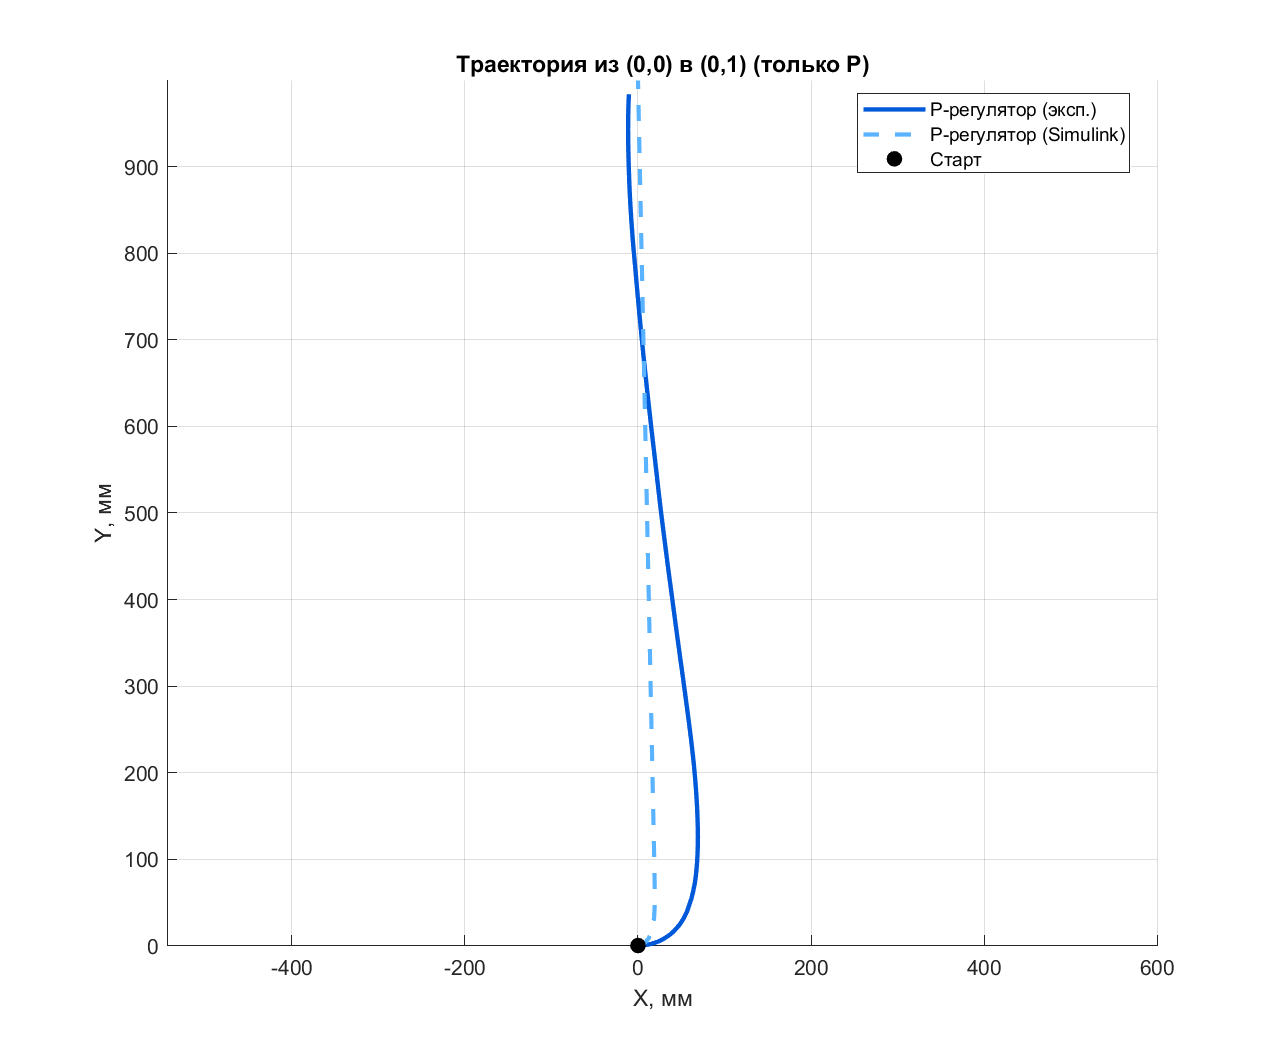
\includegraphics[width=0.82\textwidth]{../graphics/point_P_2.png}
    \caption{P-регулятор: движение из $(0,0)$ в $(0,1)$}
    \label{fig:p_only_2}
\end{figure}

При движении в точку $(0,1)$ сначала возникает заметная дуга. Это связано с тем, что робот одновременно едет вперёд и поворачивает: при большой $\alpha$ сигнал $U_r$ велик, но $U_s$ тоже остаётся ненулевым. Поэтому робот не доворачивается на месте, а входит в траекторию по кривой.

\begin{figure}[H]
    \centering
    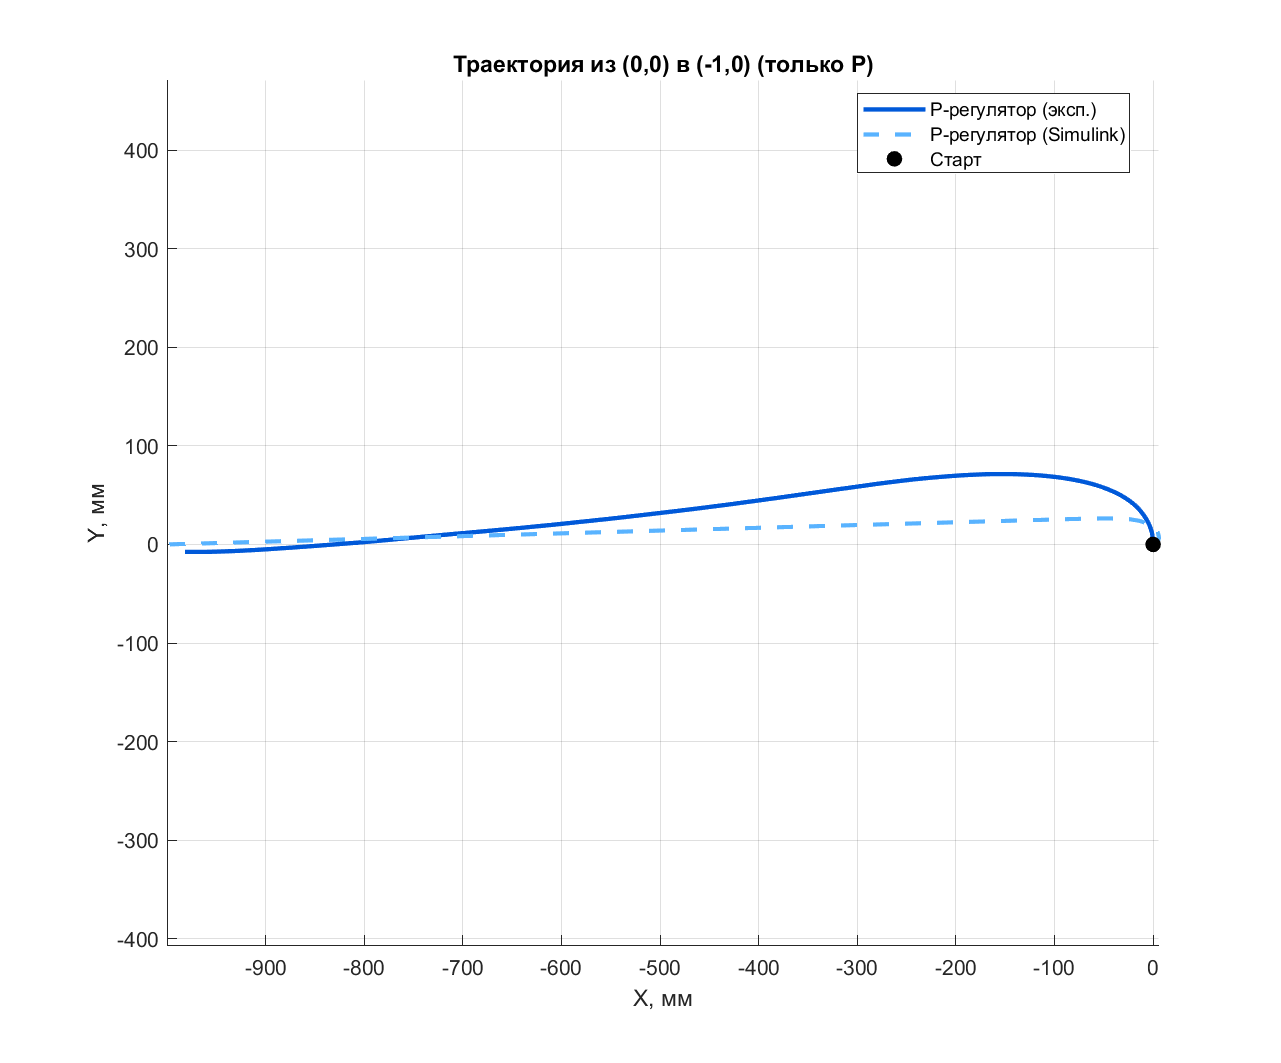
\includegraphics[width=0.82\textwidth]{../graphics/point_P_3.png}
    \caption{P-регулятор: движение из $(0,0)$ в $(-1,0)$}
    \label{fig:p_only_3}
\end{figure}

Для точки $(-1,0)$ различие формы траектории становится наибольшим. Здесь начальная угловая ошибка близка к $180^\circ$, и робот долго перестраивает курс. В результате траектория получается широкой, а влияние несимметрии моторов и ошибки одометрии усиливается.

\begin{figure}[H]
    \centering
    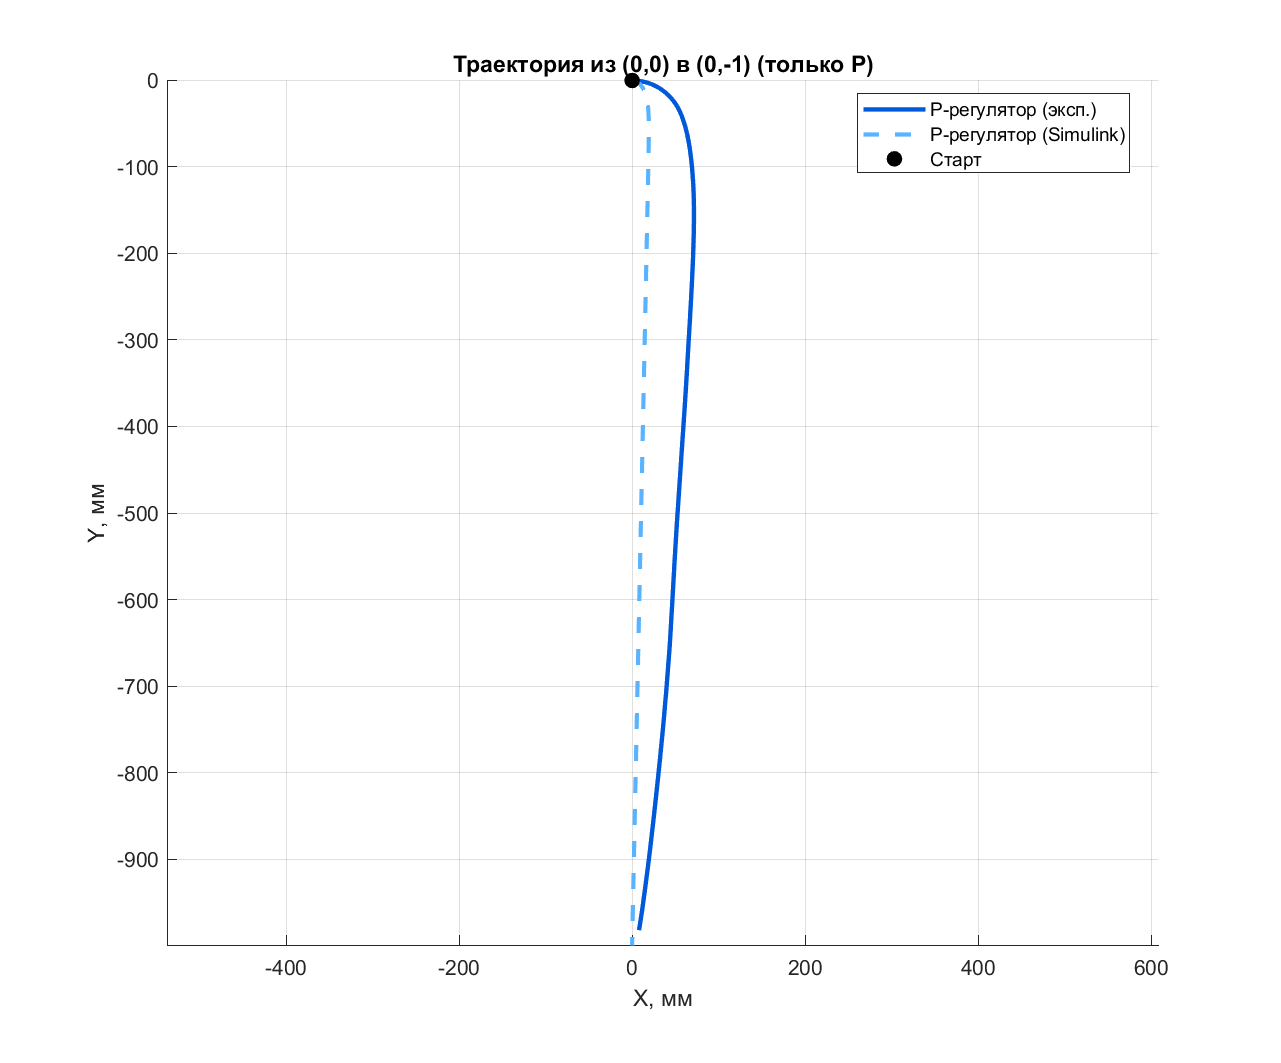
\includegraphics[width=0.82\textwidth]{../graphics/point_P_4.png}
    \caption{P-регулятор: движение из $(0,0)$ в $(0,-1)$}
    \label{fig:p_only_4}
\end{figure}

Для перехода в точку $(0,-1)$ наблюдается тот же эффект: траектория сначала изгибается, а затем выпрямляется по мере уменьшения $\alpha$. Значит, для P-регулятора характерен широкий вход в траекторию при больших начальных углах.

\subsubsection*{Сравнение траекторий P-регулятора}

\begin{figure}[H]
    \centering
    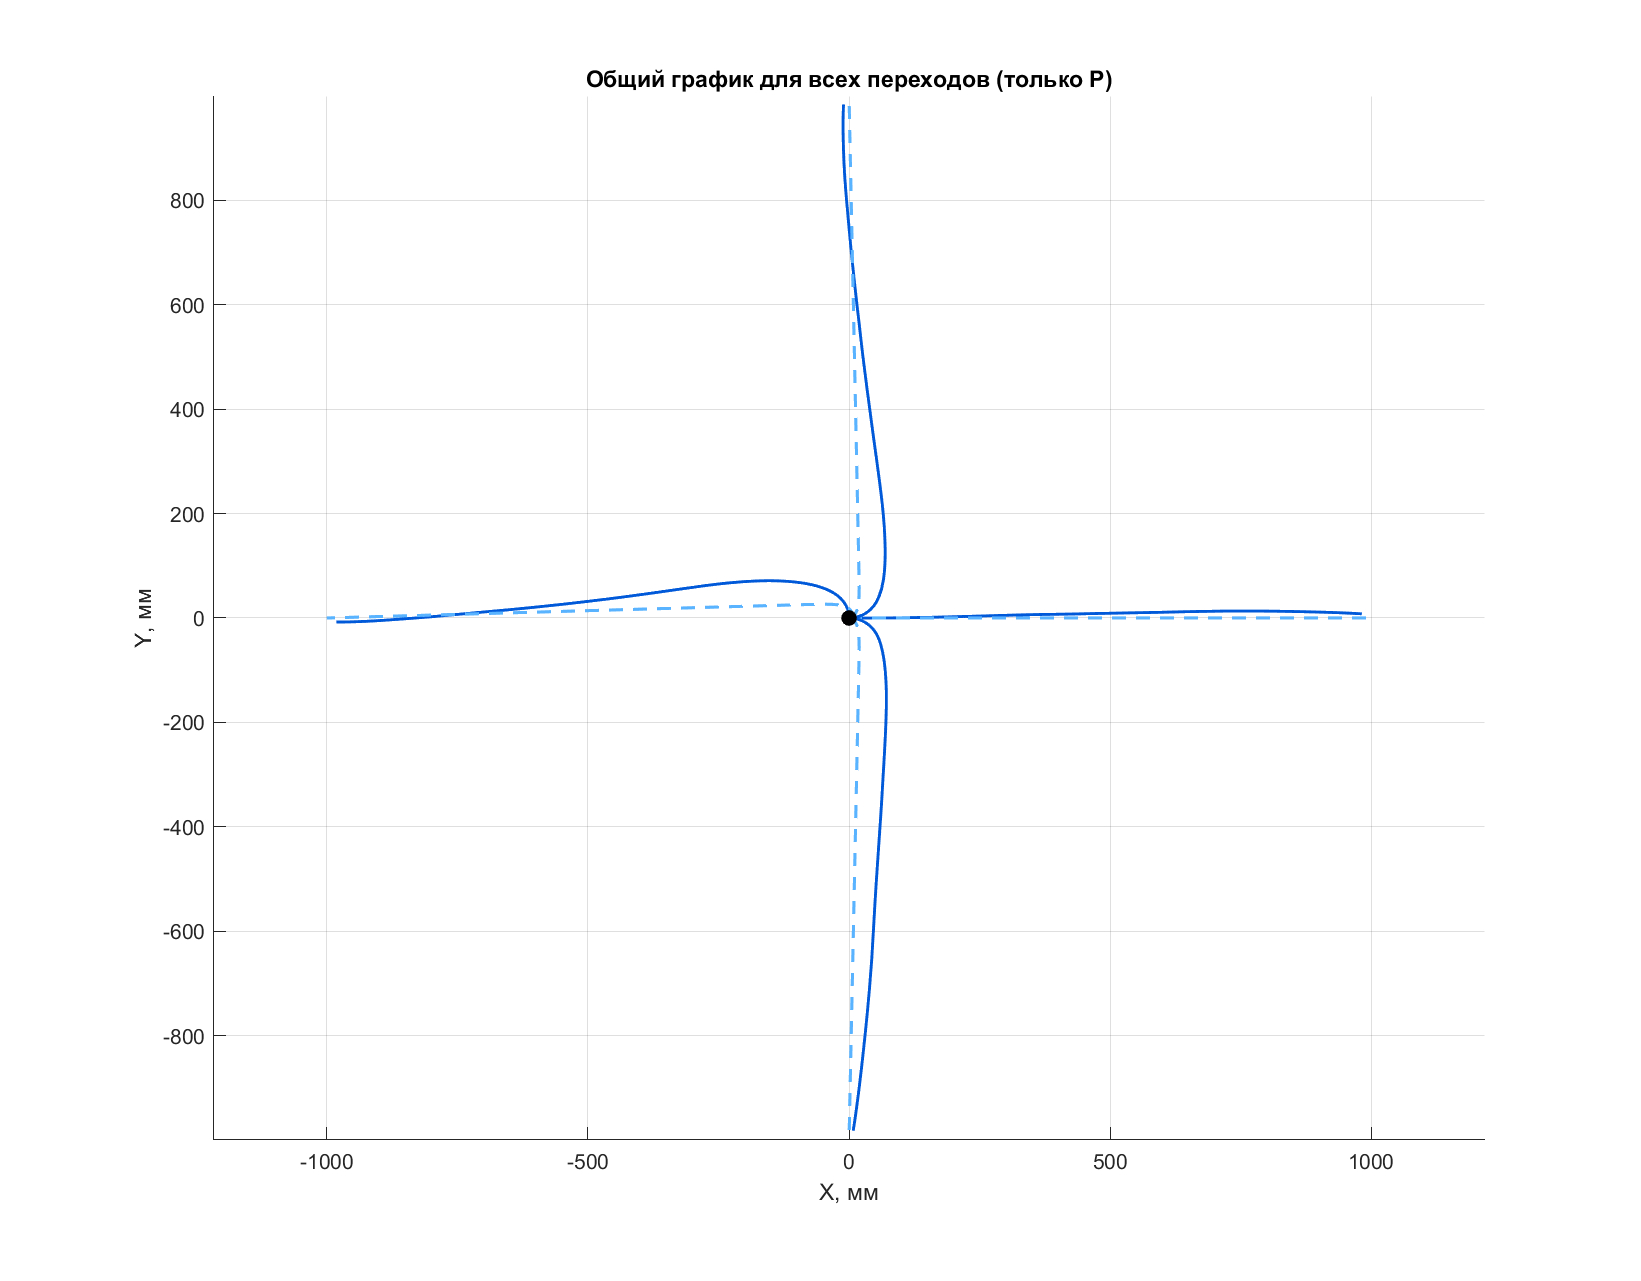
\includegraphics[width=0.9\textwidth]{../graphics/all_points_P.png}
    \caption{Все одиночные переходы для P-регулятора}
    \label{fig:all_points_p}
\end{figure}

Если сравнивать именно форму траекторий, то у P-регулятора хорошо видно общее свойство: чем больше начальный угол между направлением робота и целью, тем шире дуга. То есть различие между переходами определяется не только положением цели, но и величиной $\alpha$ в начальный момент.

\begin{figure}[H]
    \centering
    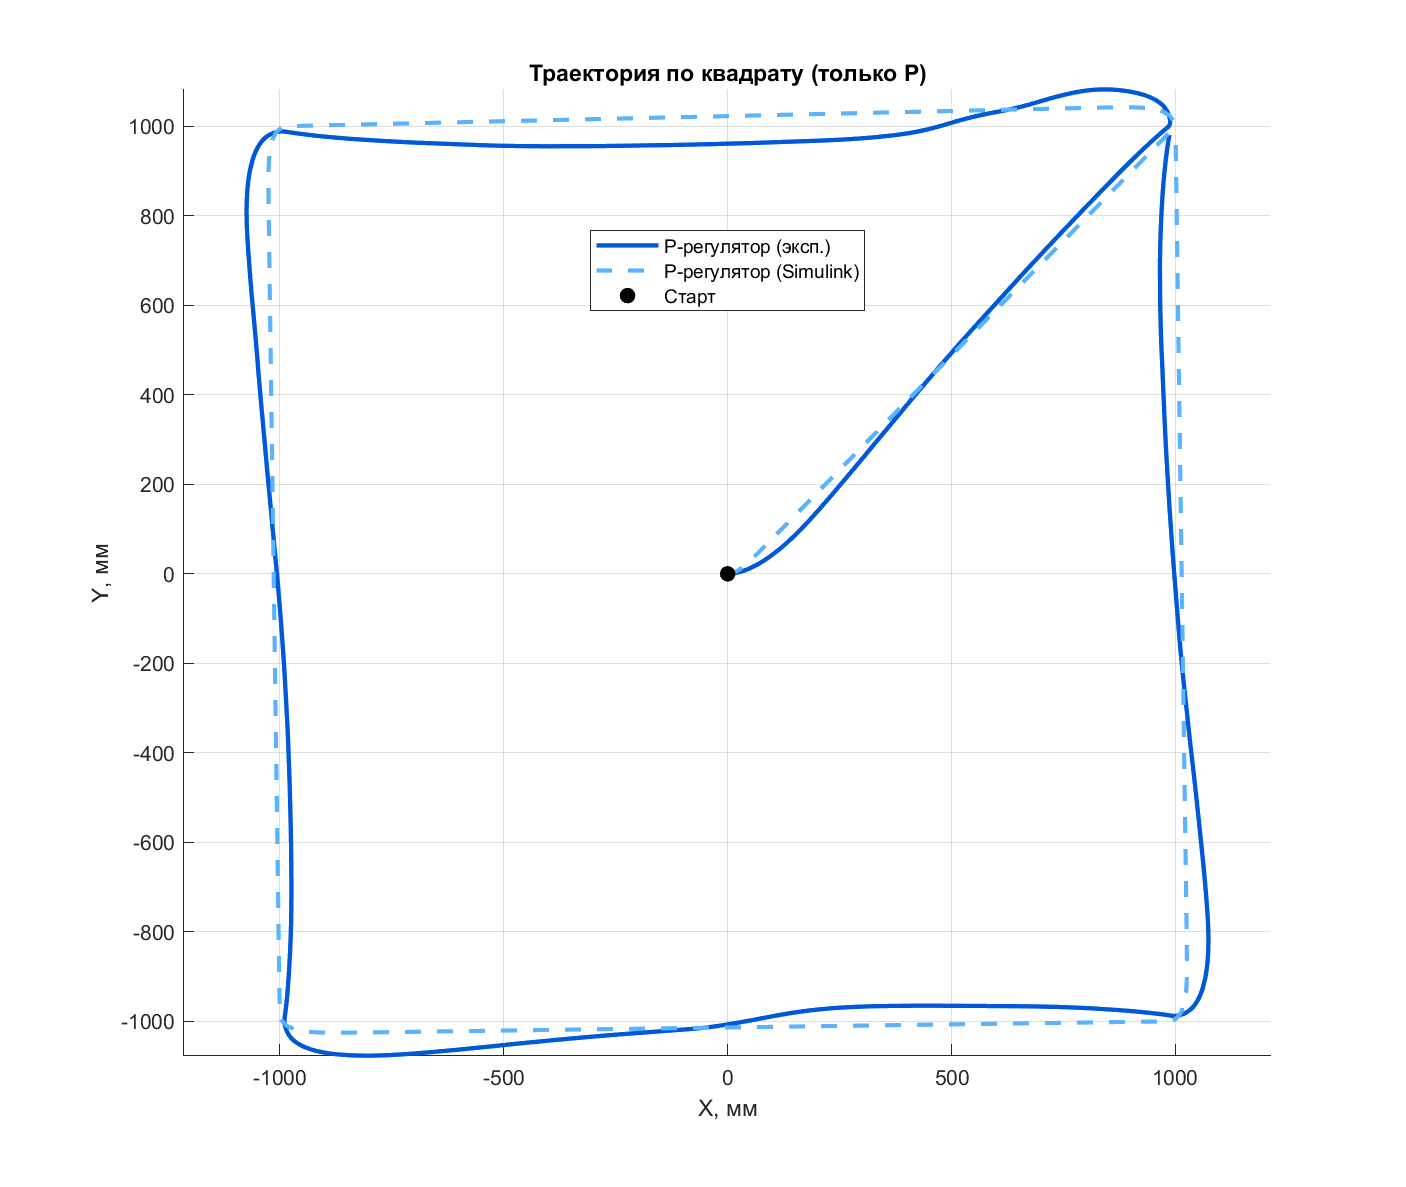
\includegraphics[width=0.84\textwidth]{../graphics/square_path_P.png}
    \caption{Движение по квадрату для P-регулятора}
    \label{fig:square_p}
\end{figure}

На квадратной траектории это проявляется особенно ясно. После каждого поворота робот входит в новую сторону не по прямой, а по сглаженной дуге. Поэтому вершины квадрата оказываются частично ``срезанными'', а после нескольких сторон появляется заметное смещение всей траектории.

\subsection{Тангенциальный регулятор}

\subsubsection*{Одиночные переходы}

\begin{figure}[H]
    \centering
    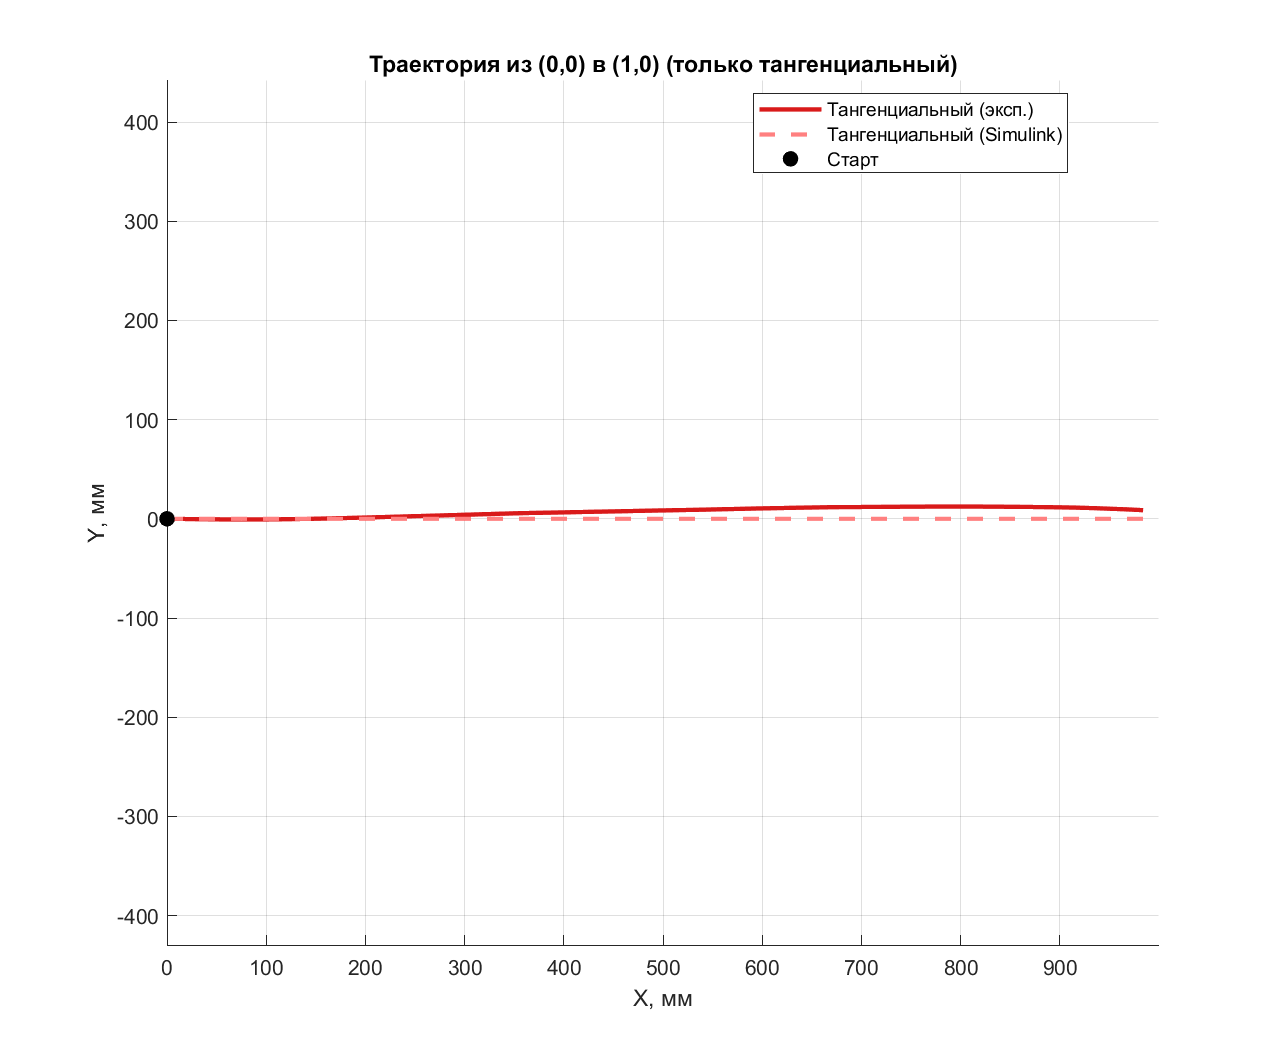
\includegraphics[width=0.82\textwidth]{../graphics/point_T_1.png}
    \caption{Тангенциальный регулятор: движение из $(0,0)$ в $(1,0)$}
    \label{fig:t_only_1}
\end{figure}

При движении в точку $(1,0)$ траектория также близка к прямой. Здесь угол ошибки мал, поэтому множитель $\cos(\alpha)$ почти не меняет линейную скорость, и оба регулятора ведут себя похоже.

\begin{figure}[H]
    \centering
    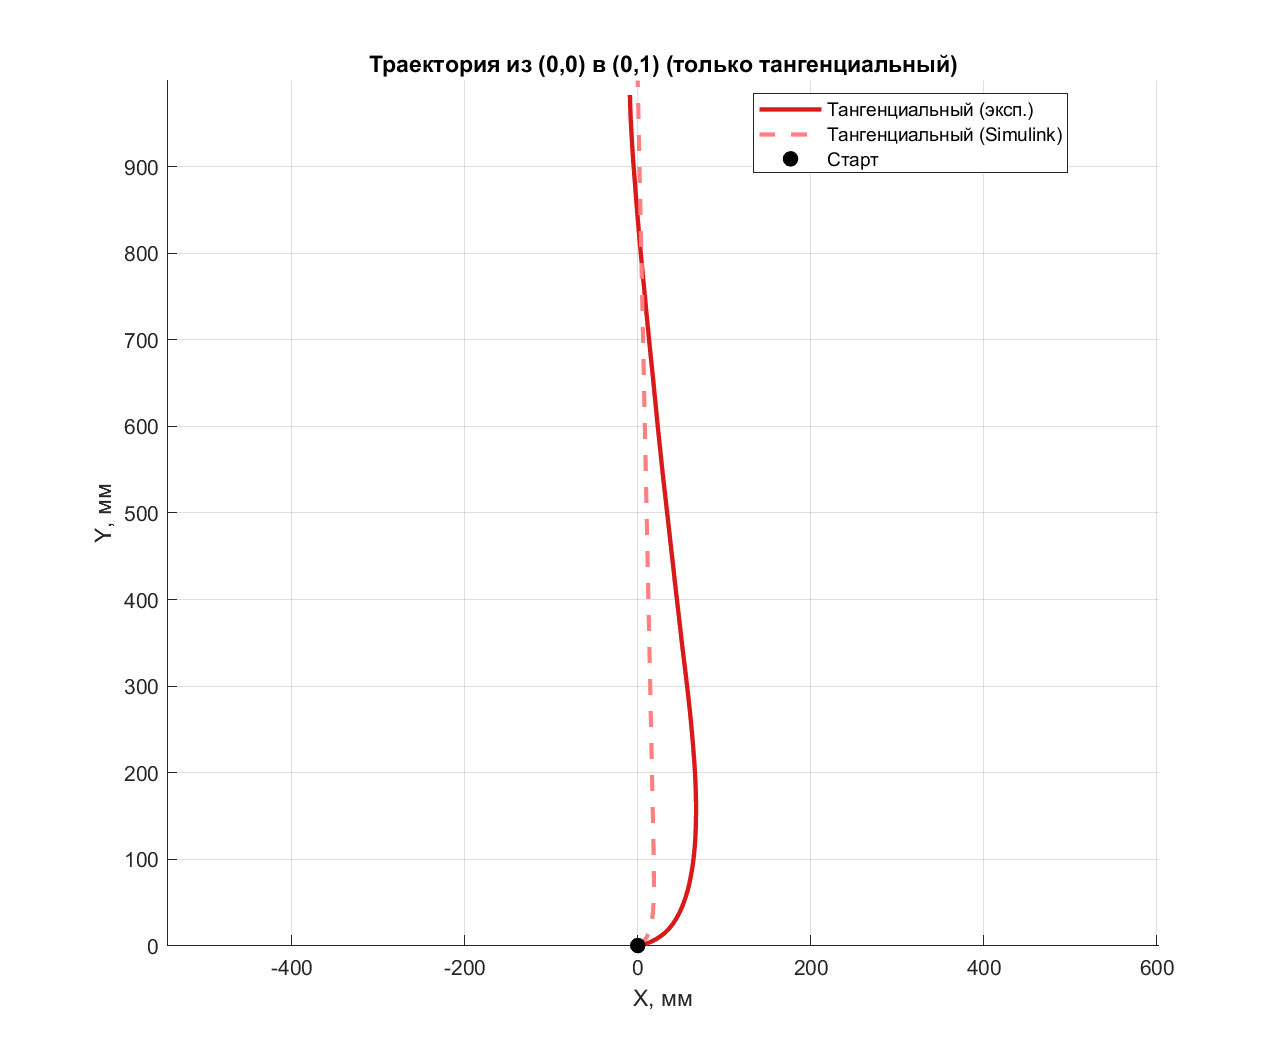
\includegraphics[width=0.82\textwidth]{../graphics/point_T_2.png}
    \caption{Тангенциальный регулятор: движение из $(0,0)$ в $(0,1)$}
    \label{fig:t_only_2}
\end{figure}

При движении в точку $(0,1)$ траектория уже заметно компактнее, чем у P-регулятора. Причина в том, что при большом $\alpha$ линейная скорость уменьшается из-за множителя $\cos(\alpha)$, и робот сначала доворачивается, а потом активнее идёт вперёд. Поэтому боковой уход меньше.

\begin{figure}[H]
    \centering
    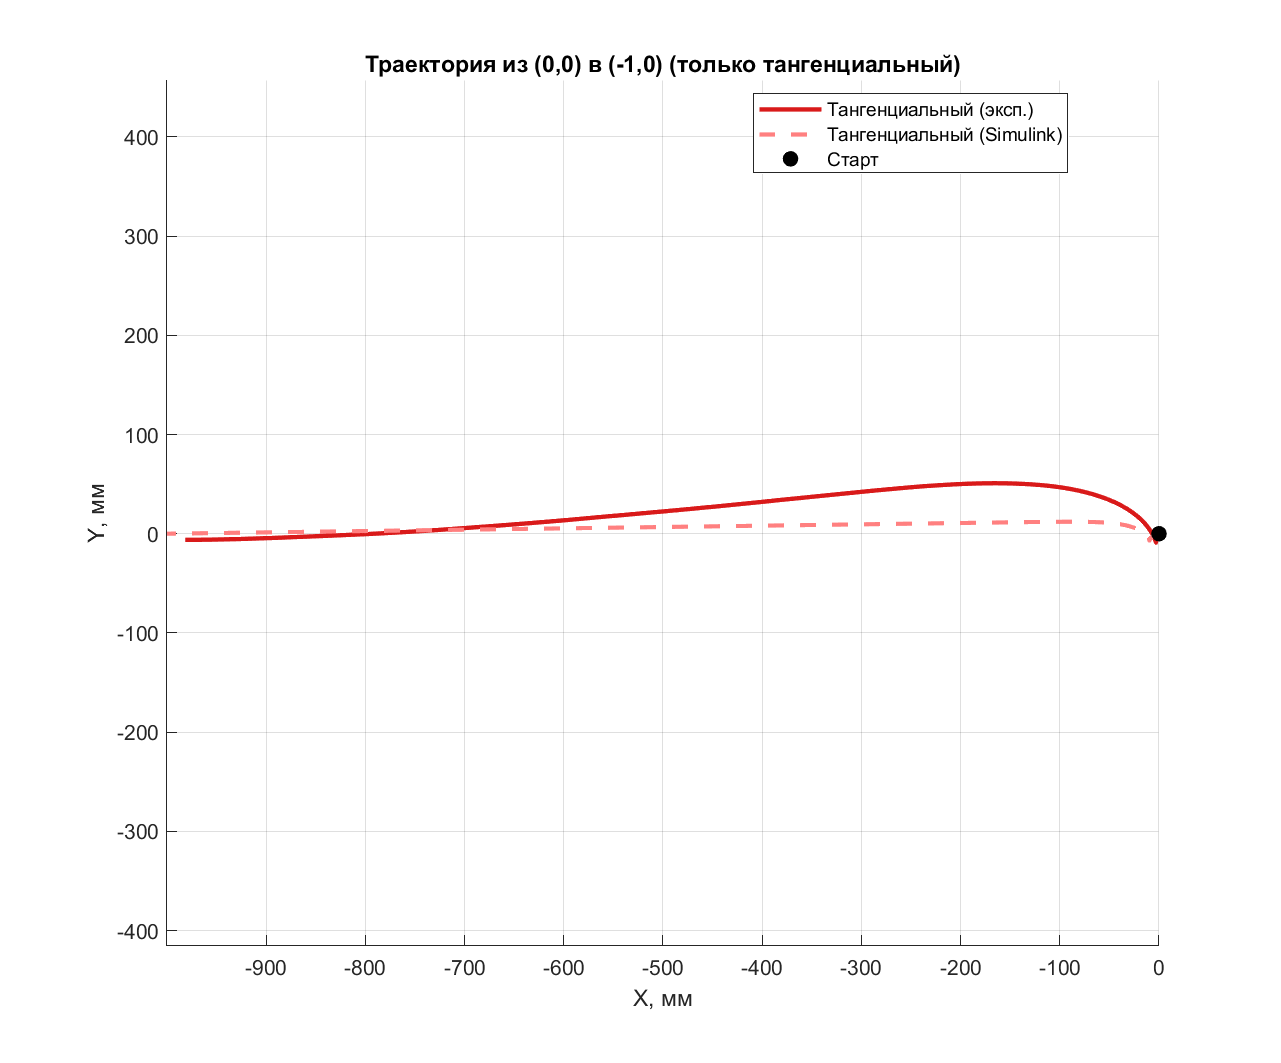
\includegraphics[width=0.82\textwidth]{../graphics/point_T_3.png}
    \caption{Тангенциальный регулятор: движение из $(0,0)$ в $(-1,0)$}
    \label{fig:t_only_3}
\end{figure}

Для точки $(-1,0)$ преимущество особенно заметно. Там, где P-регулятор строит широкую дугу, тангенциальный регулятор даёт более собранную траекторию. Это связано с тем, что при большой угловой ошибке движение вперёд подавляется, и робот меньше уходит в сторону.

\begin{figure}[H]
    \centering
    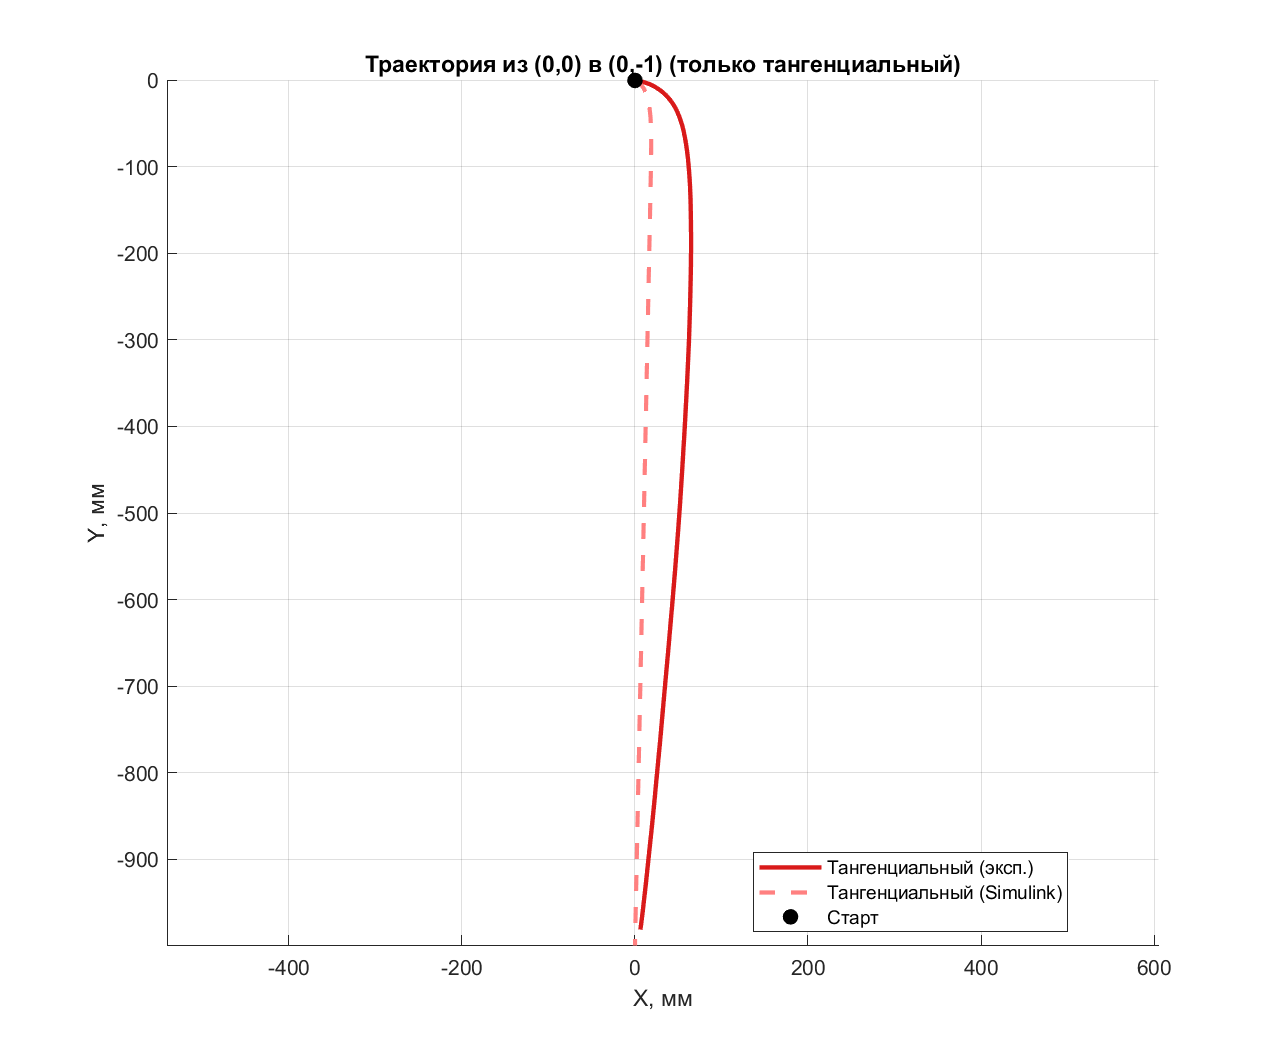
\includegraphics[width=0.82\textwidth]{../graphics/point_T_4.png}
    \caption{Тангенциальный регулятор: движение из $(0,0)$ в $(0,-1)$}
    \label{fig:t_only_4}
\end{figure}

При переходе в точку $(0,-1)$ наблюдается тот же эффект. Траектория остаётся более узкой, а вход в направление к цели происходит быстрее. Это значит, что тангенциальный регулятор лучше работает в случаях большого начального углового рассогласования.

\subsubsection*{Сравнение траекторий тангенциального регулятора}

\begin{figure}[H]
    \centering
    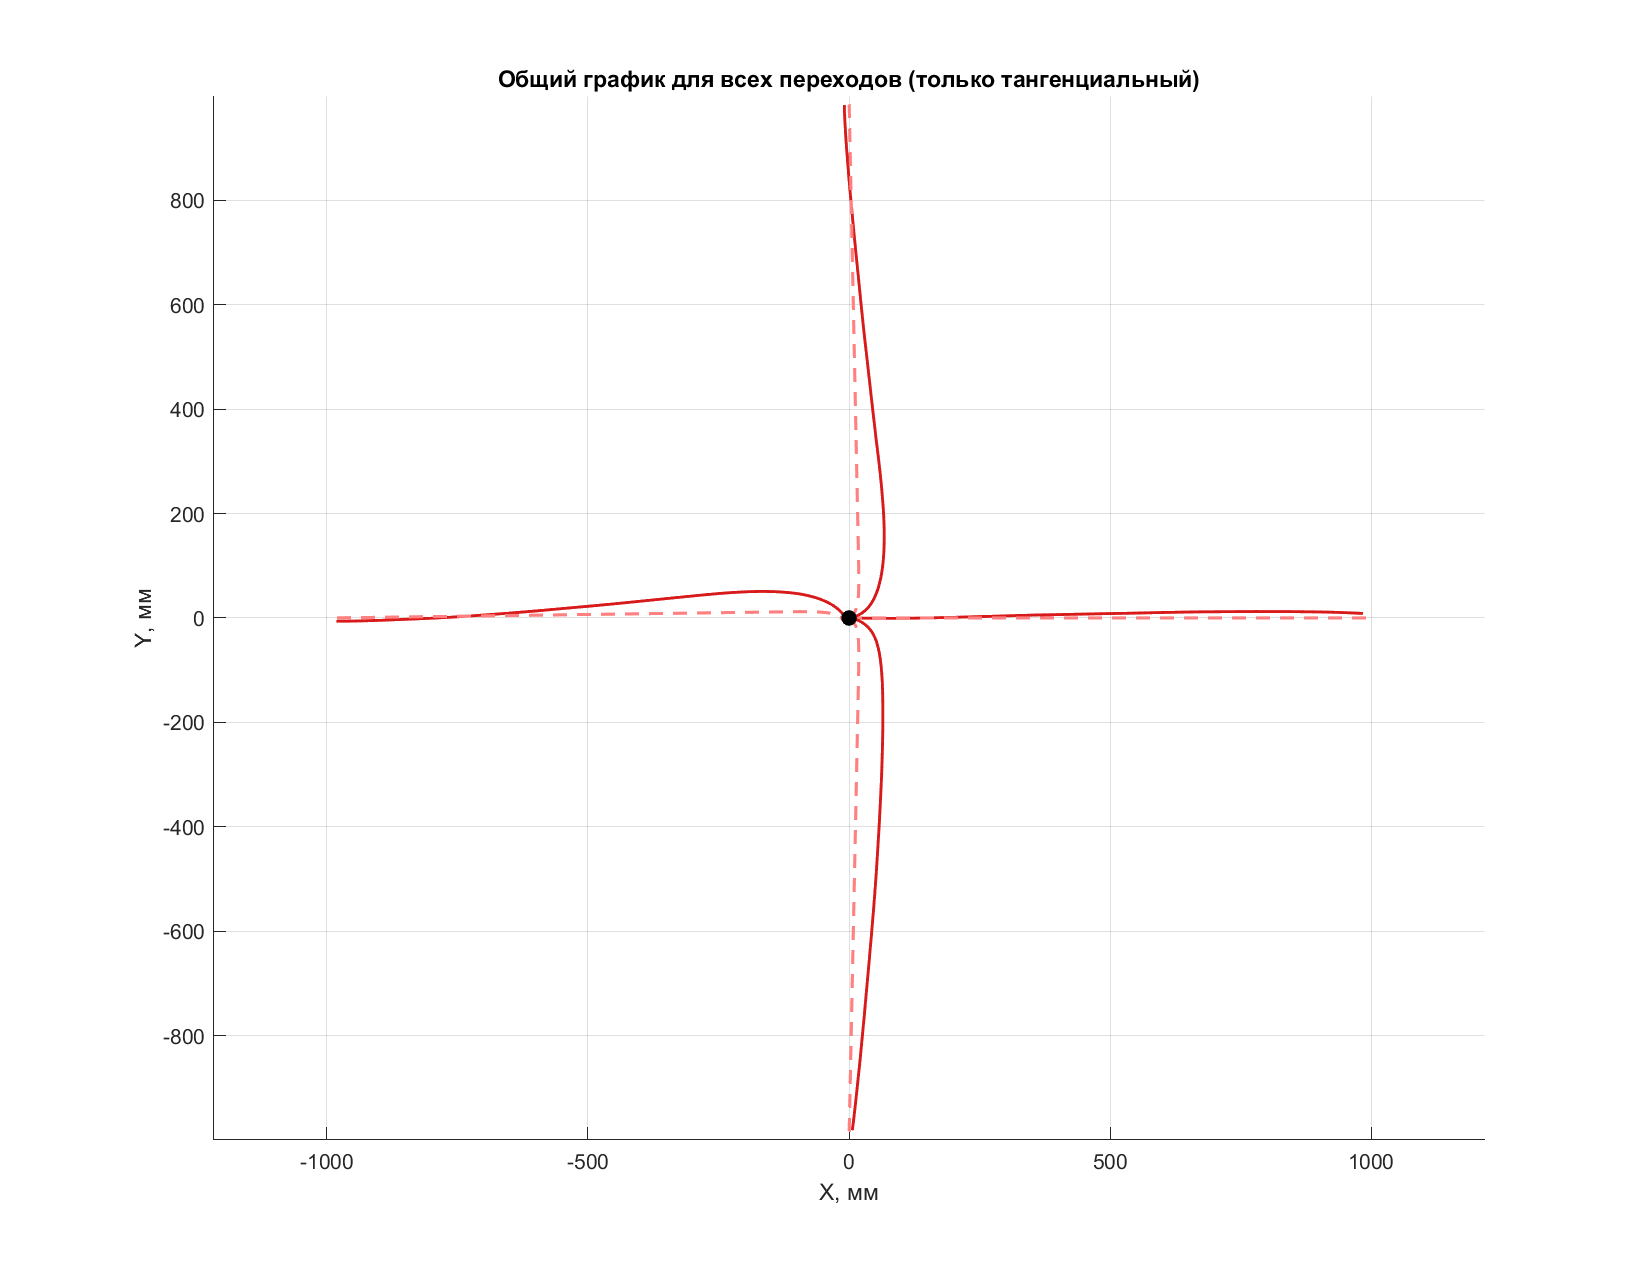
\includegraphics[width=0.9\textwidth]{../graphics/all_points_T.png}
    \caption{Все одиночные переходы для тангенциального регулятора}
    \label{fig:all_points_t}
\end{figure}

Если сравнивать именно форму траекторий, то у тангенциального регулятора они менее растянуты вбок и ближе друг к другу по характеру. Это означает, что регулятор слабее зависит от начального угла и лучше сохраняет структуру движения при разных положениях цели.

\begin{figure}[H]
    \centering
    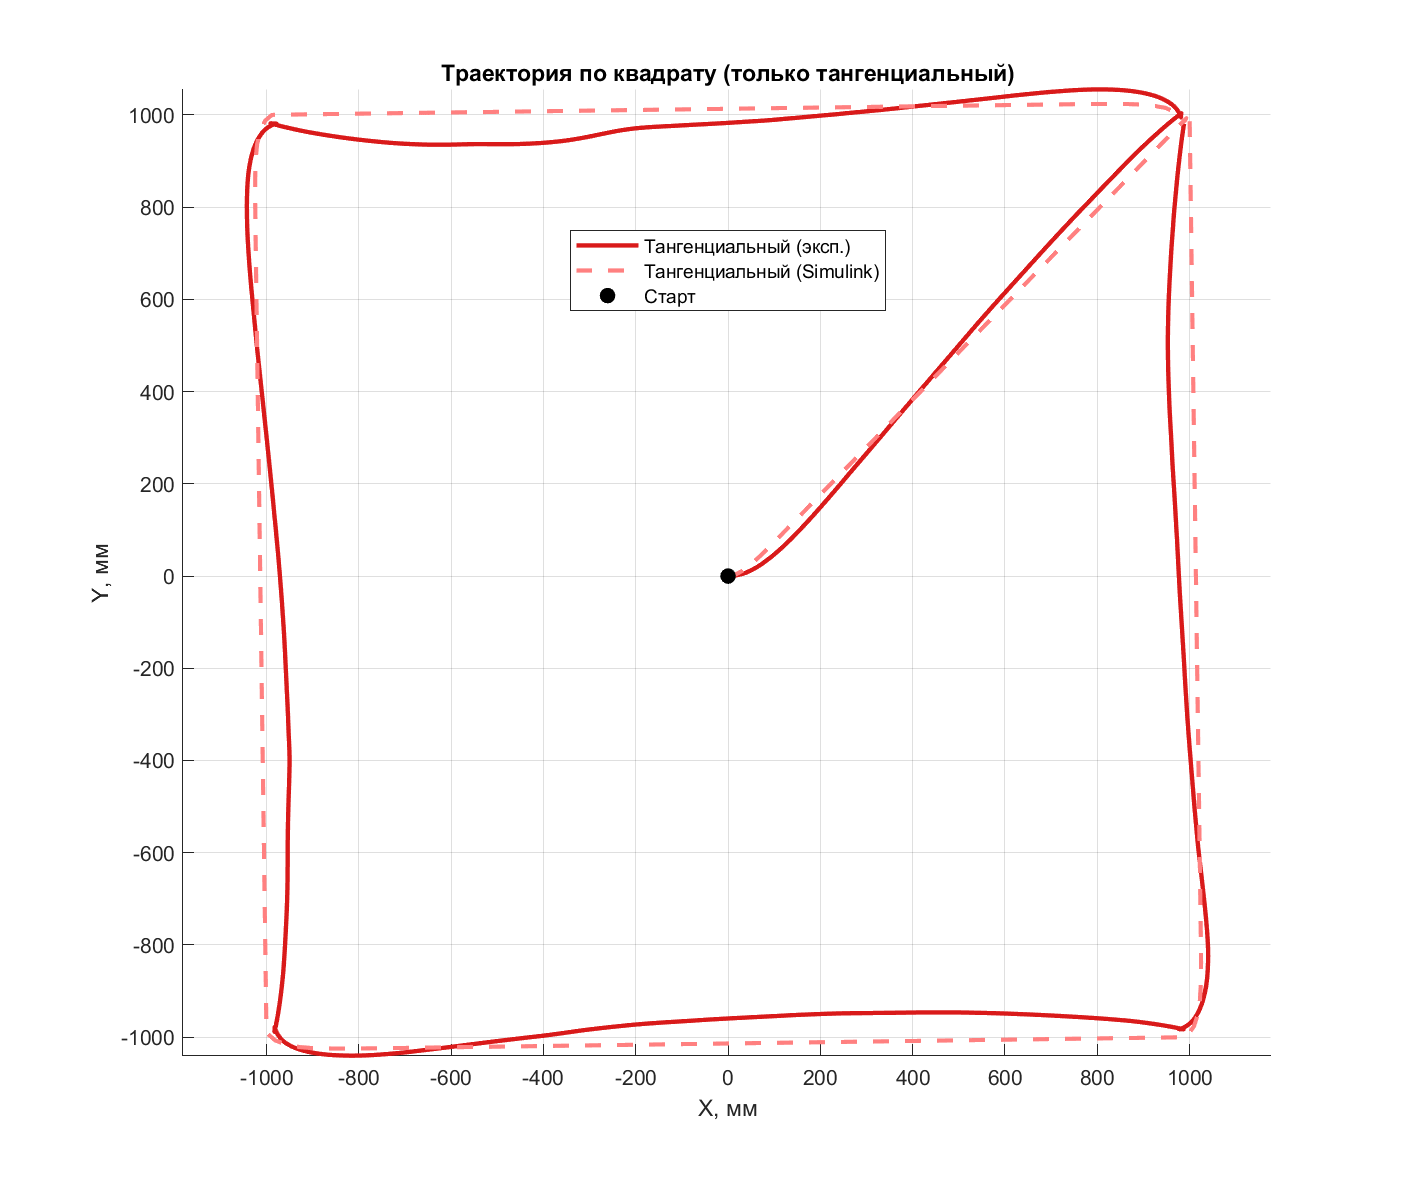
\includegraphics[width=0.84\textwidth]{../graphics/square_path_T.png}
    \caption{Движение по квадрату для тангенциального регулятора}
    \label{fig:square_t}
\end{figure}

На квадратной траектории повороты между сторонами получаются короче по переходному участку. Вершины тоже не идеальны, но они выражены лучше, чем у P-регулятора. Значит, при последовательных манёврах тангенциальный закон управления лучше сохраняет форму заданной траектории.

\subsection{Общее сравнение регуляторов}

\subsubsection*{Сравнение для отдельных переходов}

\begin{figure}[H]
    \centering
    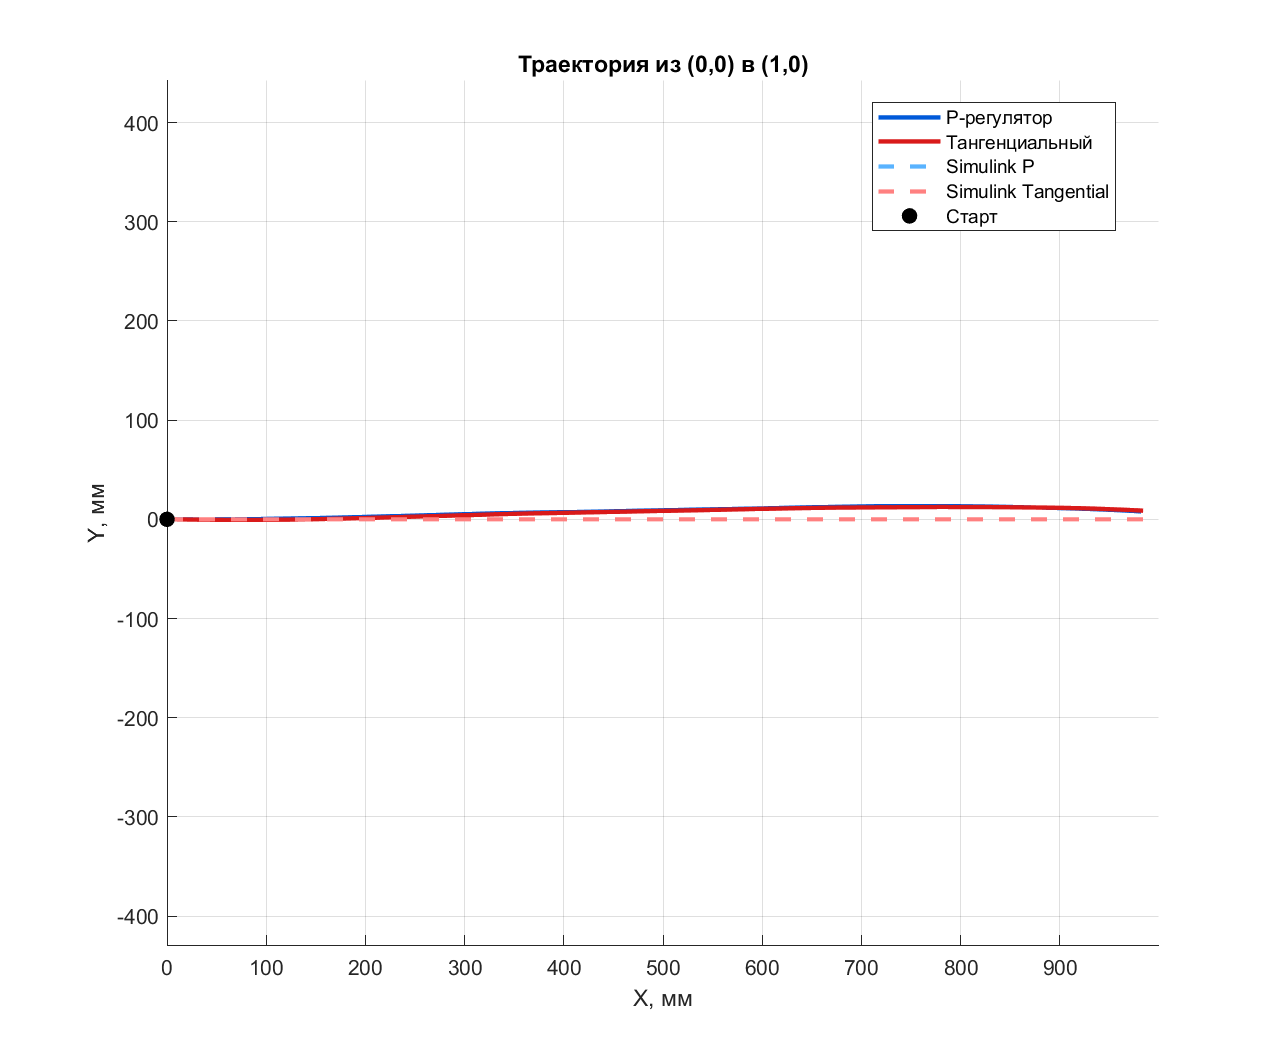
\includegraphics[width=0.82\textwidth]{../graphics/point_1.png}
    \caption{Сравнение двух регуляторов при движении в точку $(1,0)$}
    \label{fig:point_1_common}
\end{figure}

В случае движения в точку $(1,0)$ оба регулятора дают близкий результат. Здесь задача самая простая, поэтому преимущества более сложного закона управления выражены слабо.

\begin{figure}[H]
    \centering
    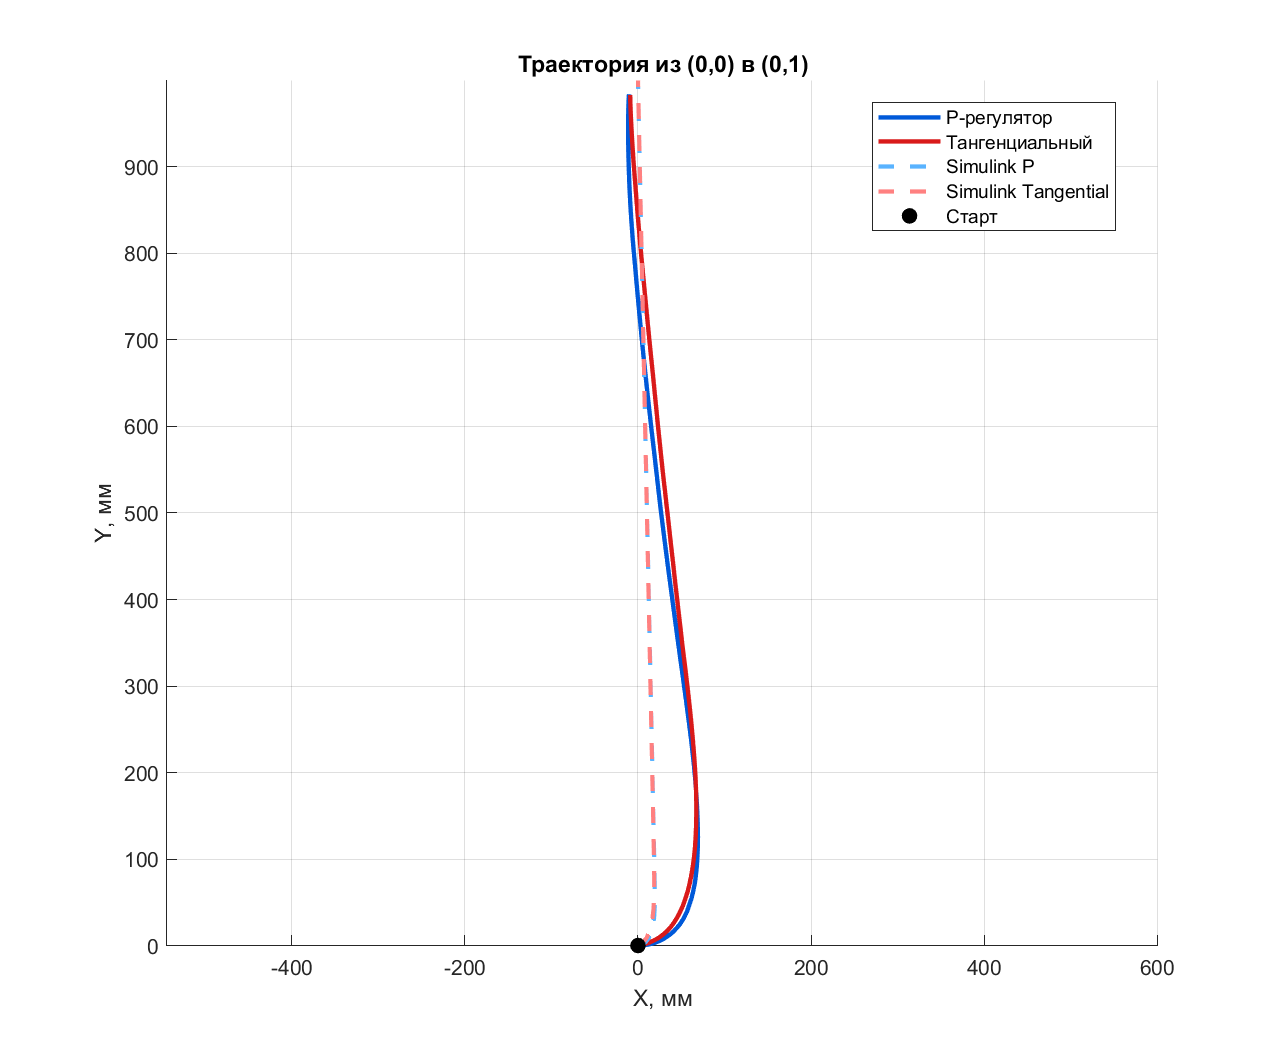
\includegraphics[width=0.82\textwidth]{../graphics/point_2.png}
    \caption{Сравнение двух регуляторов при движении в точку $(0,1)$}
    \label{fig:point_2_common}
\end{figure}

При переходе в точку $(0,1)$ разница уже заметнее. Тангенциальный регулятор строит более узкую траекторию и меньше уходит в сторону на этапе выхода к цели.

\begin{figure}[H]
    \centering
    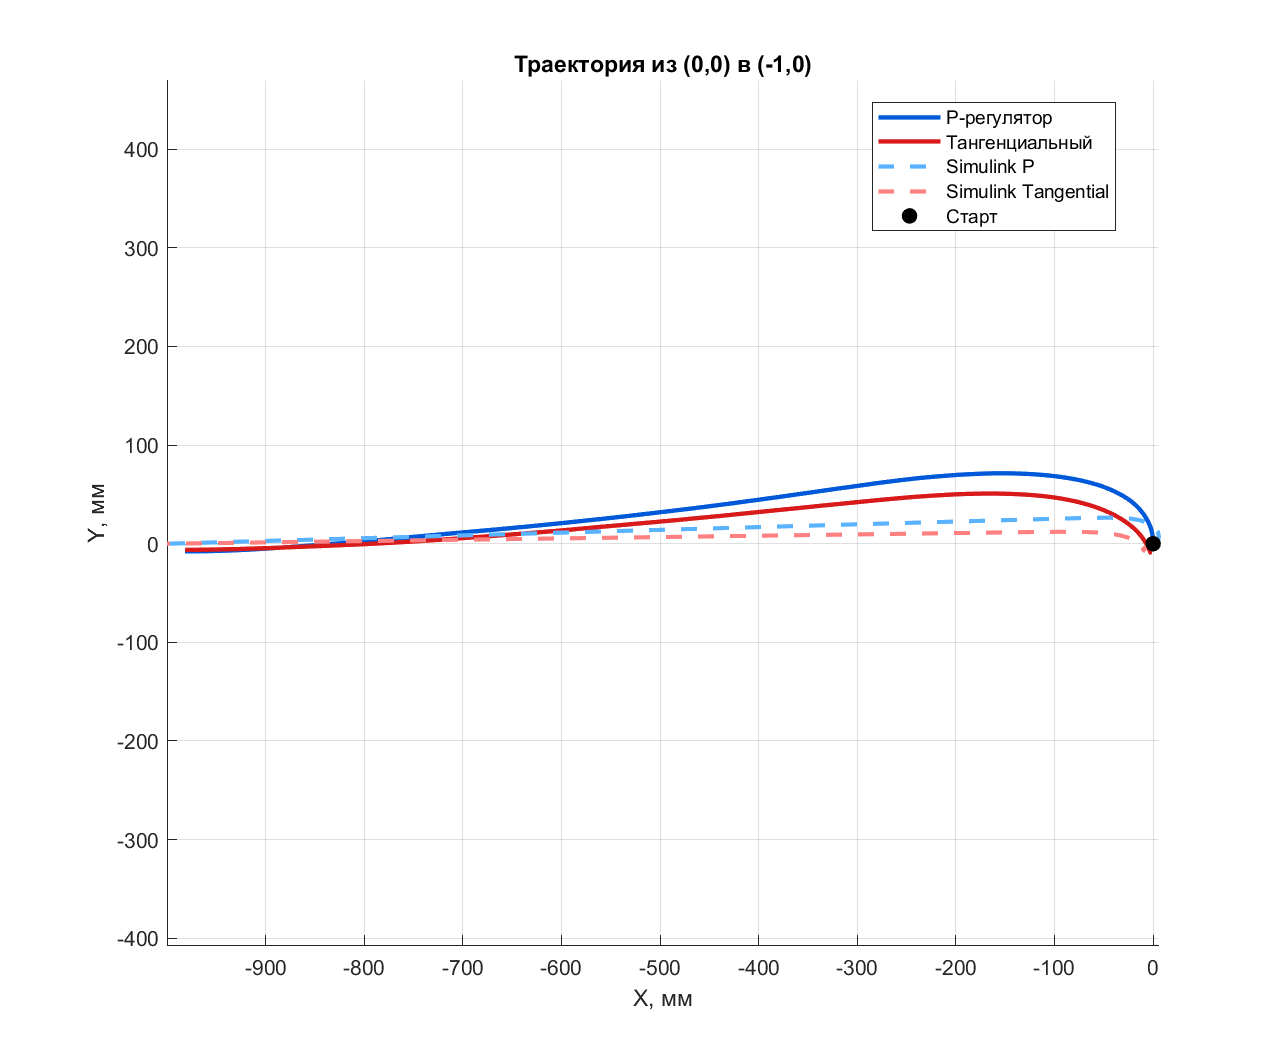
\includegraphics[width=0.82\textwidth]{../graphics/point_3.png}
    \caption{Сравнение двух регуляторов при движении в точку $(-1,0)$}
    \label{fig:point_3_common}
\end{figure}

Для цели позади начального положения преимущество тангенциального регулятора выражено наиболее сильно. Он лучше справляется с большими начальными угловыми ошибками и реже формирует слишком широкую дугу.

\begin{figure}[H]
    \centering
    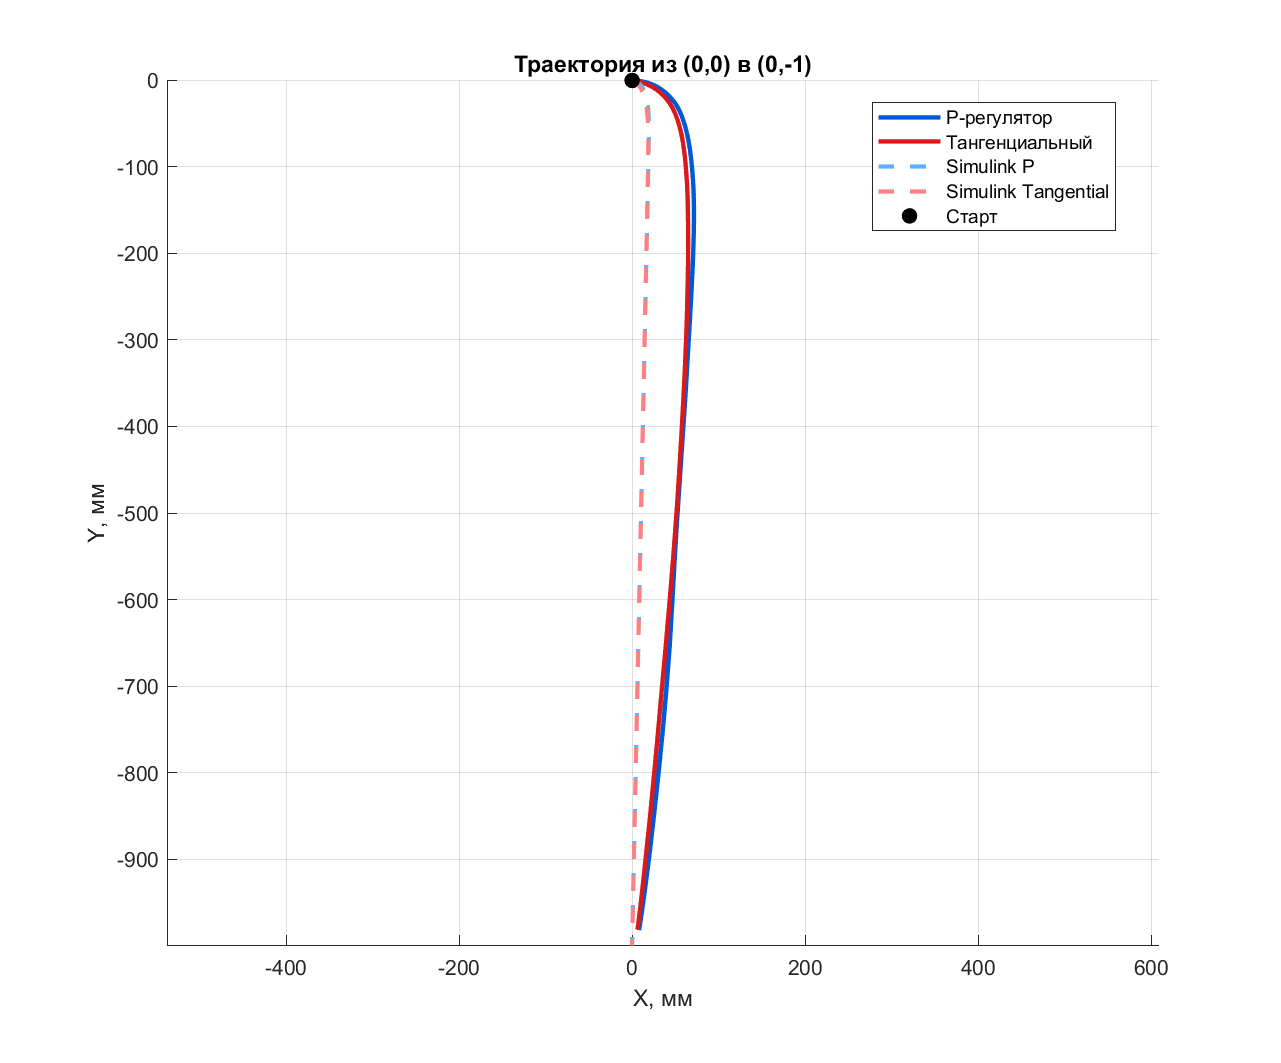
\includegraphics[width=0.82\textwidth]{../graphics/point_4.png}
    \caption{Сравнение двух регуляторов при движении в точку $(0,-1)$}
    \label{fig:point_4_common}
\end{figure}

Случай $(0,-1)$ даёт такой же вывод. Оба регулятора решают задачу, но тангенциальный делает это более аккуратно по форме траектории.

\subsubsection*{Сравнение формы траекторий}

Если сравнивать регуляторы именно по форме траекторий, то главное различие состоит в следующем: у P-регулятора траектория чаще начинается широкой дугой, а у тангенциального регулятора --- более коротким участком доворота с меньшим боковым уходом. Это особенно хорошо видно для целей $(0,1)$, $(-1,0)$ и $(0,-1)$, где начальная ошибка по углу велика.

Математически это объясняется структурой законов управления. У P-регулятора поступательное движение определяется как $U_s = K_s \rho$, то есть зависит только от расстояния до цели и не уменьшается само по себе при большой угловой ошибке. Поэтому робот продолжает ехать вперёд даже тогда, когда ещё не довёрнут к цели. У тангенциального регулятора линейная скорость содержит множитель $\cos(\alpha)$, поэтому при больших значениях $\alpha$ движение вперёд уменьшается. Именно из-за этого его траектория обычно уже и ближе к направлению на цель.

Для последовательного движения по квадрату это различие становится ещё заметнее. У P-регулятора каждая новая сторона начинается с более длинного переходного дугового участка, поэтому форма квадрата постепенно искажается. У тангенциального регулятора переход между сторонами короче, поэтому общая траектория лучше сохраняет геометрию маршрута.

\subsubsection*{Сравнение всех одиночных переходов}

\begin{figure}[H]
    \centering
    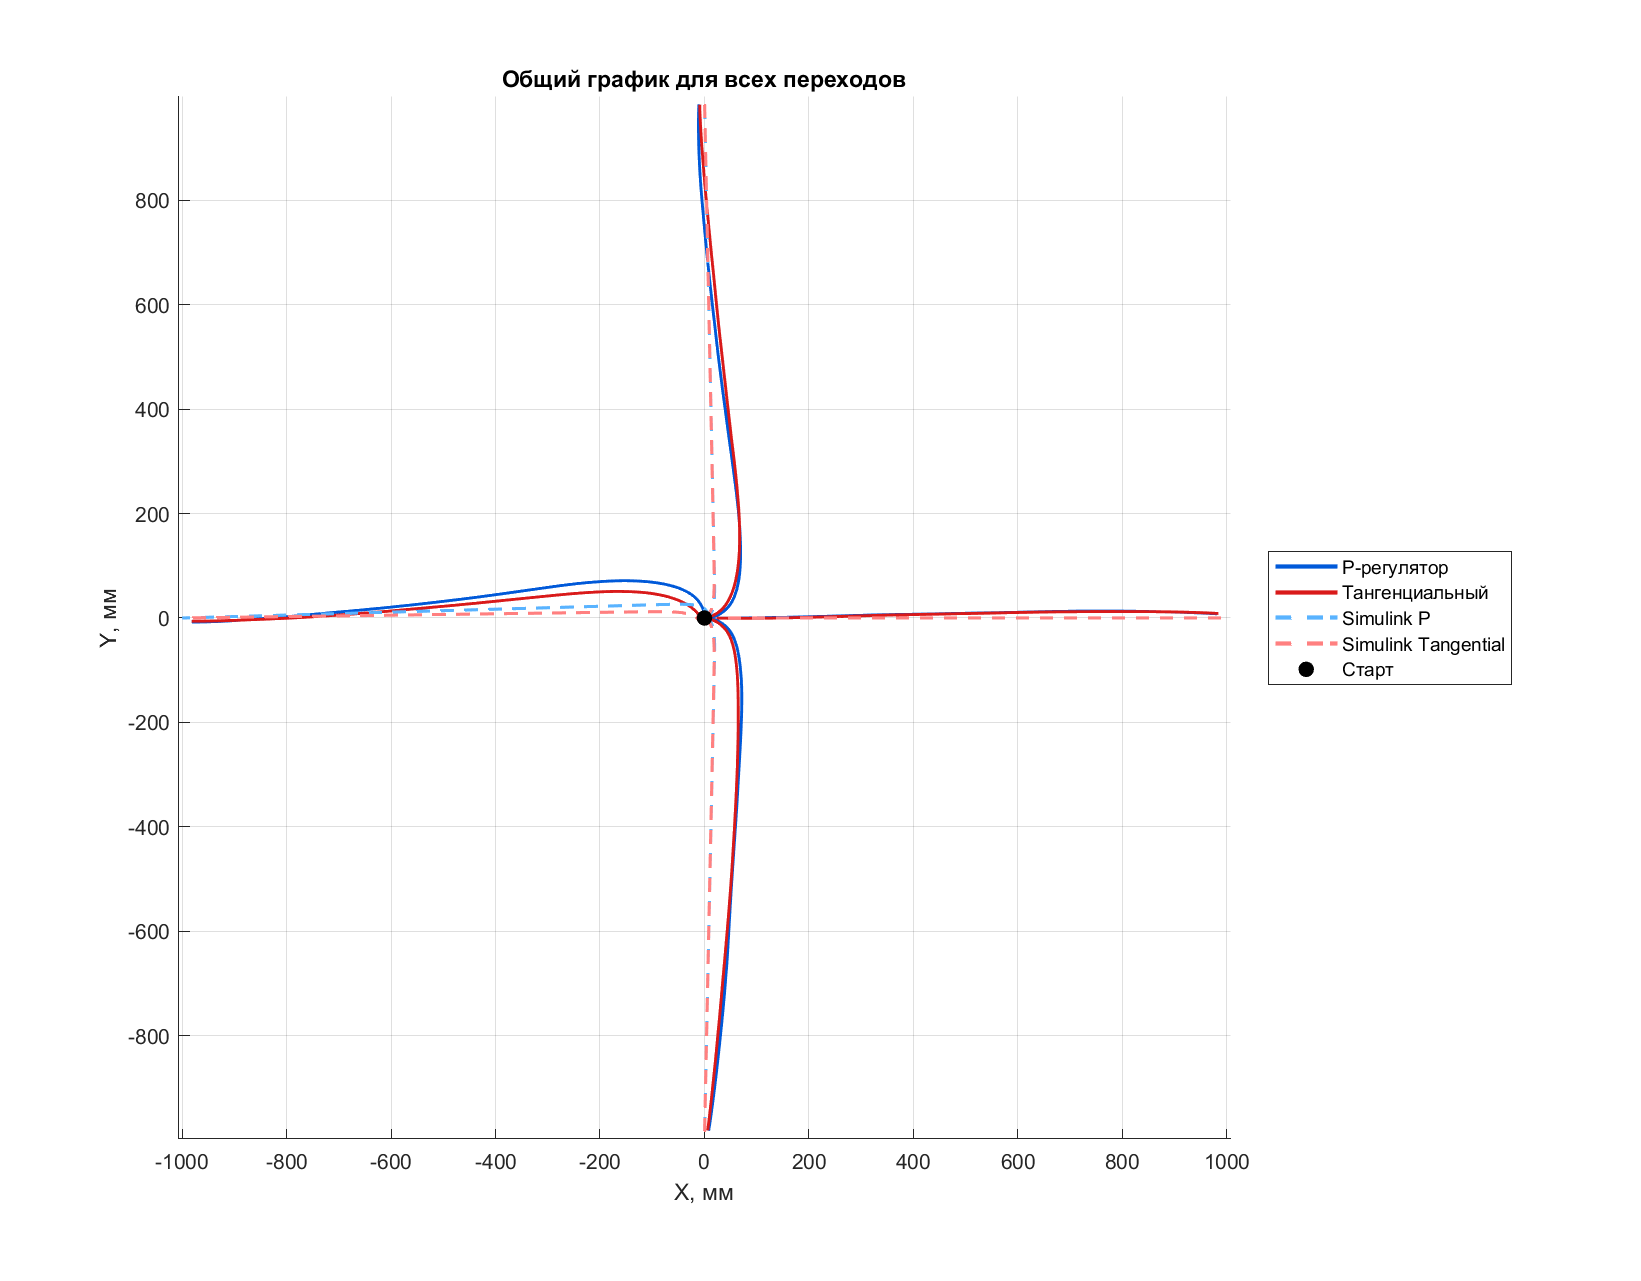
\includegraphics[width=0.95\textwidth]{../graphics/all_points.png}
    \caption{Общий график всех одиночных переходов}
    \label{fig:all_points_common}
\end{figure}

На этом графике видно, что в простых переходах разница между регуляторами невелика, а в переходах с сильным разворотом траектории тангенциального регулятора оказываются компактнее. Значит, его преимущество проявляется прежде всего в более сложной геометрии движения.

\subsubsection*{Сравнение движения по квадрату}

\begin{figure}[H]
    \centering
    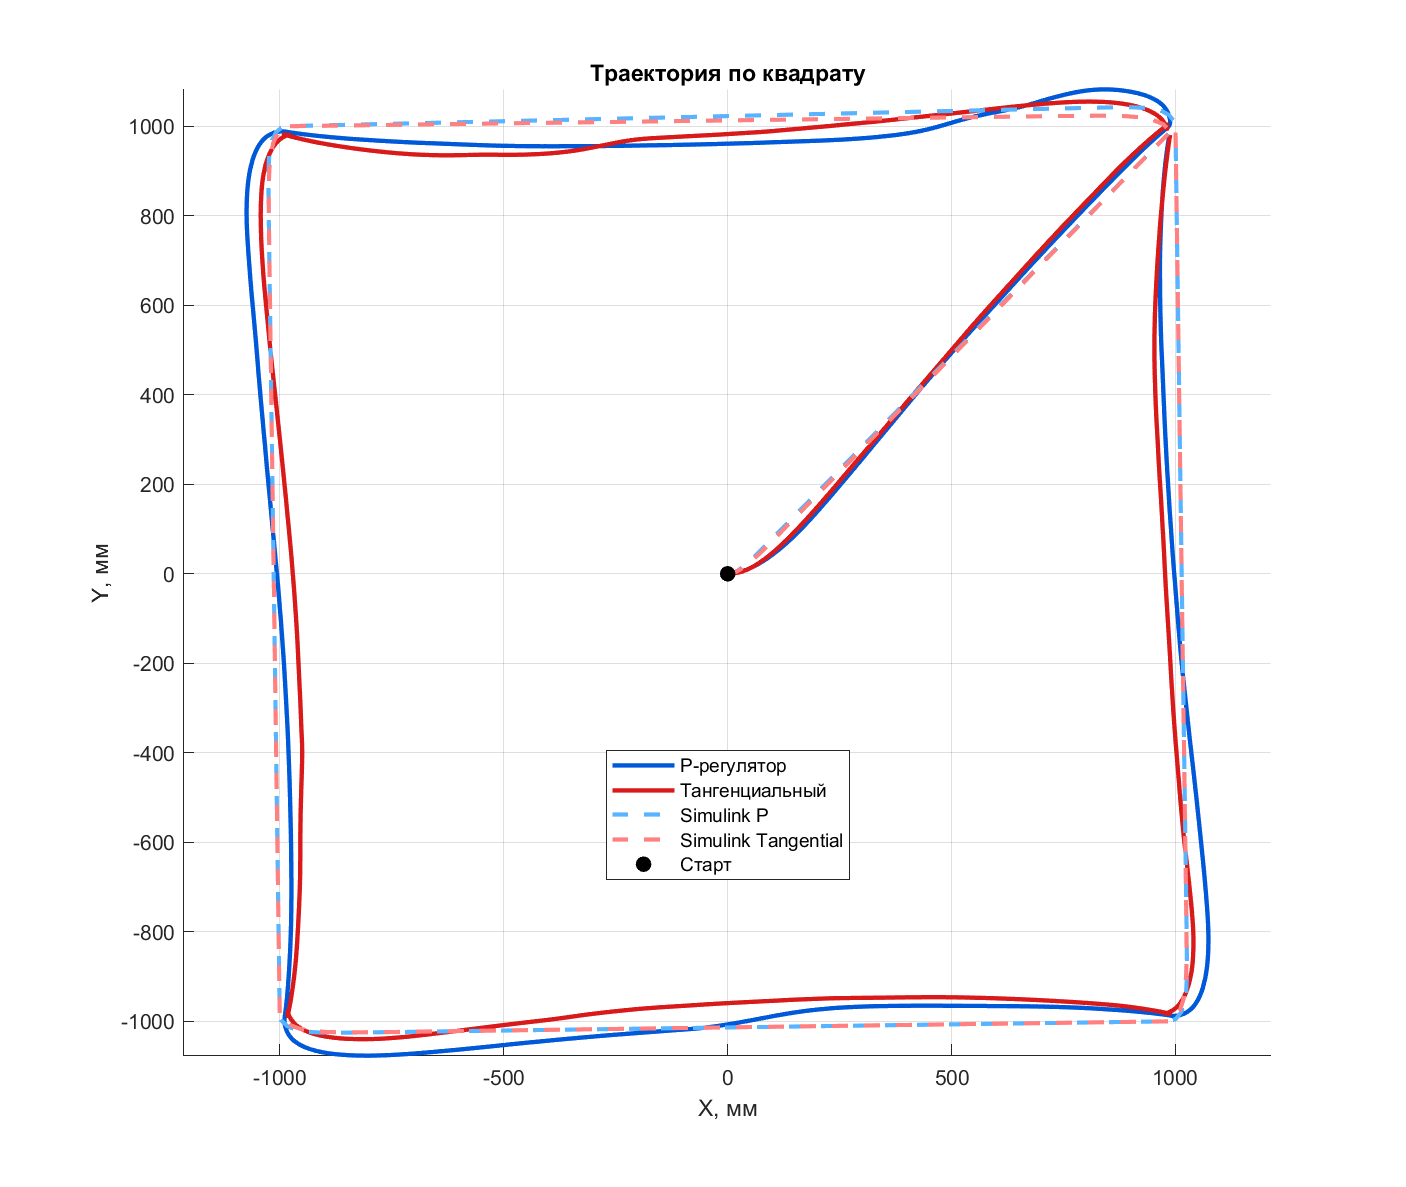
\includegraphics[width=0.88\textwidth]{../graphics/square_path.png}
    \caption{Сравнение двух регуляторов при движении по квадрату}
    \label{fig:square_common}
\end{figure}

Движение по квадрату является самым показательным испытанием, потому что здесь одновременно присутствуют прямолинейные участки, развороты и накопление ошибки от шага к шагу. На этом графике видно, что тангенциальный регулятор в среднем лучше сохраняет форму траектории, а P-регулятор сильнее искажает квадрат после нескольких последовательных поворотов.

\section{Анализ различий между моделью и экспериментом}

Расхождения между моделью и экспериментом связаны не с одной причиной, а с наложением нескольких факторов.

Во-первых, модель является кинематической. В ней предполагается, что заданный сигнал сразу приводит к нужной скорости колёс. В реальном роботе моторы имеют инерцию и не выходят мгновенно на требуемый режим. Поэтому в начале движения и при поворотах экспериментальная траектория отличается от расчётной.

Во-вторых, в модели левое и правое колёса считаются полностью одинаковыми, а база робота --- постоянной. В реальной конструкции даже небольшая асимметрия колёс, различие трения или смещение центра масс приводит к систематическому отклонению. На длинной траектории эта ошибка накапливается.

В-третьих, сравнение выполняется по данным одометрии, а не по внешнему измерению координат. Значит, часть расхождения связана не только с движением робота, но и с ошибкой оценки его положения. Особенно сильно это проявляется на квадратной траектории, где ошибка каждой стороны переходит на следующую.

В-четвёртых, различие определяется и самим видом регулятора. У P-регулятора движение вперёд не ослабляется при большой угловой ошибке, поэтому траектория получается более широкой. У тангенциального регулятора линейная скорость уменьшается через множитель $\cos(\alpha)$, поэтому робот сначала лучше ориентируется на цель и только потом активнее движется вперёд.

Следовательно, различие между моделью и экспериментом объясняется совместным действием упрощённой кинематики, ошибки одометрии, неидеальности моторов и различной структуры законов управления. Именно поэтому тангенциальный регулятор в эксперименте обычно даёт более компактные траектории, хотя полного совпадения с моделью всё равно не возникает.

\section{Заключение}

В работе были построены и исследованы два способа управления роботом с дифференциальным приводом: P-регулятор и тангенциальный регулятор. Для обоих случаев были собраны модели в Simulink, проведены эксперименты на роботе EV3 и построены графики одиночных переходов и движения по квадрату.

Главный результат состоит в том, что оба регулятора решают задачу вывода робота в целевую точку, но формируют разные траектории. P-регулятор даёт более широкие дуги при больших начальных углах, потому что движение вперёд сохраняется даже при большой ошибке ориентации. Тангенциальный регулятор формирует более компактные траектории, так как его линейная скорость уменьшается при росте угловой ошибки.

Сравнение с экспериментом показало, что кинематическая модель правильно передаёт общий характер движения, но не описывает его полностью. Основные трудности были связаны с накоплением ошибки одометрии, неидеальностью моторов и тем, что реальный робот реагирует на управление не так, как идеализированная модель. Практическая ценность работы состоит в том, что удалось не только реализовать управление и моделирование, но и понять, как структура регулятора влияет на форму траектории реального мобильного робота.

\appendix
\section{Листинг программы на Python}
\lstinputlisting[language=Python]{../prog/main.py}

\section{Листинг Matlab-скрипта}
\lstinputlisting[language=Matlab]{../matlab/run_all_litle.m}

\end{document}